% !TeX encoding = utf8
% !TeX program = pdflatex
% !TeX spellcheck = de-DE	

% Titelseite muss NICHT verändert werden! Nur die \work packages in preamble/misc anpassen

% ========================================================================
\documentclass[
    a4paper,                           % !DIN A4 paper
    twoside, openright
    fontsize=12pt,					% default font size
    titlepage,						% title page environment
    numbers=noenddot,				% headline numbering without dot	
    parskip=half,					% Absatz halbe Zeile Abstand (mit -,+,*, modifizierbar)
    abstracton,
    toc = bibiography,
]{scrreprt}							% !KOMA-script Klasse (scrreprt, scrartcl, scrbook)

% ======================== PREAMBEL ========================
% ==========================================================
% ========================================================================
\usepackage[utf8]{inputenc}							% !UTF-8
%
% ~~~~~~~~~~~~~~~~~~~~~~~~~~~~~~~~~~~~~~~~~~~~~~~~~~~~~~~~~~~~~~~~~~~~~~~~
% 1. Einige Pakete müssen vor allen anderen geladen werden
% ~~~~~~~~~~~~~~~~~~~~~~~~~~~~~~~~~~~~~~~~~~~~~~~~~~~~~~~~~~~~~~~~~~~~~~~~
\usepackage{xspace} 								% Define commands that don't eat spaces.
\usepackage[ngerman]{babel}					% Languagesetting: Sprachpaket wird in \documentclass für gesamtes Dokument festgelegt

\usepackage[hyperref]{xcolor} 			% benutzerdefinierte Farben
\usepackage[]{graphicx} 	 					% für Bilder
%\usepackage[fleqn]{amsmath}					% Amsmath - Mathematik Basispaket fl=flush left = linksbündig
\usepackage{amsmath}                            % Amsmath - Mathematik Basispaket zentriert
\usepackage{tikz}		    						% für Graphiken und Zeichnen
\usepackage{pgfplots}								% Für MATLAB2Latex export



% ~~~~~~~~~~~~~~~~~~~~~~~~~~~~~~~~~~~~~~~~~~~~~~~~~~~~~~~~~~~~~~~~~~~~~~~~
% Fonts und Seitenränder
% ~~~~~~~~~~~~~~~~~~~~~~~~~~~~~~~~~~~~~~~~~~~~~~~~~~~~~~~~~~~~~~~~~~~~~~~~
\usepackage[T1]{fontenc} 							% T1 Schrift Encoding (notwendig für die meisten Type 1 Schriften)
\usepackage{textcomp}
\usepackage{lmodern}


\usepackage[            
	left=3.5cm,										% linke Randbreite                                                                     
	right=2cm,										% rechte Randbreite                                                                  
	top=2.7cm,										% oberer Rand                                                                         
	bottom=3cm									% unterer Rand
]{geometry}											% Seitenlayout verändern                    

%%%% Head and Footline
\usepackage[
	headsepline,
	plainheadsepline,
	automark,
]{scrlayer-scrpage}
\addtokomafont{pagehead}{\normalfont \sffamily}
\chead*{} 
%\ohead*{\headmark}
%\automark{chapter}
\ofoot*{\pagemark} 
\cfoot*{}        

%% Inhaltsverzeichnis

\usepackage{tocloft}

\renewcommand{\cftchapfont}{\subsectionfont}
\renewcommand{\cftsecfont}{\subsectionfont}
\renewcommand{\cftsubsecfont}{\subsectionfont}

\renewcommand{\cftchappagefont}{\numberfont}
\renewcommand{\cftsecpagefont}{\numberfont}
\renewcommand{\cftsubsecpagefont}{\numberfont}

\renewcommand{\cftpartleader}{\cftdotfill{\cftdotsep}} % for parts
\renewcommand{\cftchapleader}{\cftdotfill{\cftdotsep}} % for chapters

\setlength{\cftbeforechapskip}{3pt}

%\usepackage{tocstyle}  Die folgenden 3 Zeilen mussten auskommentiert werden. Welche Auswirkungen das hat, weiß ich nicht.
%\settocfeature[toc][0]{entryhook}{}                                                                
%\settocfeature[0]{entryvskip}{0.5em plus 1pt}
% ~~~~~~~~~~~~~~~~~~~~~~~~~~~~~~~~~~~~~~~~~~~~~~~~~~~~~~~~~~~~~~~~~~~~~~~~                                  
% 3. Text related packages                                                                                  
% ~~~~~~~~~~~~~~~~~~~~~~~~~~~~~~~~~~~~~~~~~~~~~~~~~~~~~~~~~~~~~~~~~~~~~~~~                                  
\usepackage[hyphens]{url} 							% Setzen von URLs. In Verbindung mit hyperref sind diese auch aktive Links.
                                                                                                         
% ~~~~~~~~~~~~~~~~~~~~~~~~~~~~~~~~~~~~~~~~~~~~~~~~~~~~~~~~~~~~~~~~~~~~~~~~                                  
% 4. PDF related packages                                                                                   
% ~~~~~~~~~~~~~~~~~~~~~~~~~~~~~~~~~~~~~~~~~~~~~~~~~~~~~~~~~~~~~~~~~~~~~~~~                                  
\usepackage[                                                                                      
	colorlinks=true,	        						% Links erhalten Farben statt Kaestchen                                      
	urlcolor=black,
	filecolor=black, 
	linkcolor=black, 
	citecolor=black,                                                               
]{hyperref}											% Aktivierung für Referenzen zur Erstellung der pdf                                   
                                                   
% ~~~~~~~~~~~~~~~~~~~~~~~~~~~~~~~~~~~~~~~~~~~~~~~~~~~~~~~~~~~~~~~~~~~~~~~~                                  
% 5. Tables (Tabular)                                                                                       
% ~~~~~~~~~~~~~~~~~~~~~~~~~~~~~~~~~~~~~~~~~~~~~~~~~~~~~~~~~~~~~~~~~~~~~~~~
\usepackage{booktabs}								% horizontale Linien in Tabellen
\usepackage{multirow}								% Um in Tabellen über mehrere Zeilen gleichzeitig schreiben zu können
\usepackage{longtable}              % Tabellen über mehrere Seiten          
                                                                                                           
% ~~~~~~~~~~~~~~~~~~~~~~~~~~~~~~~~~~~~~~~~~~~~~~~~~~~~~~~~~~~~~~~~~~~~~~~~                                  
% 7. Figures and placement                                                                                  
% ~~~~~~~~~~~~~~~~~~~~~~~~~~~~~~~~~~~~~~~~~~~~~~~~~~~~~~~~~~~~~~~~~~~~~~~~                                  
\graphicspath{{fig/}}								% Pfad für Bilder. Kann im folgenden Dokument dann weggelassen werden          
\usepackage{float}									% Stellt die Option [H] für Floats zur Verfgung:\begin{figure}[H]
                                                                                                   
%========================== Zeilenabstand ================================                                  
\usepackage{setspace}								% Zeilenabstand festlegen; generell oder im Fließtext mit Befehl               
%\doublespacing	        							% 2-facher Abstand                                                             
%\onehalfspacing  									% 1,5-facher Abstand                                                              
%\singlespacing										% 1-facher Abstand                                                                 
                                                                                                         
%==================== Captions (Schrift, Aussehen) =======================
\usepackage{caption}								% Aussehen der Captions
\captionsetup{
	margin = 10pt,
	font = {small,rm},
	labelfont = {small,bf, sf},
	format = plain, 								% oder 'hang'
	indention = 0em,	 							% Einruecken der Beschriftung
	labelsep = colon, 								%period, space, quad, newline
	justification = RaggedRight, 					% justified, centering
	singlelinecheck = true, 						% false (true=bei einer Zeile immer zentrieren)
	position = bottom 								% top
}
%%% Bugfix Workaround
\DeclareCaptionOption{parskip}[]{}
\DeclareCaptionOption{parindent}[]{}
% Aussehen der Captions fuer subfigures (subfig-Paket)
\captionsetup[subfloat]{
	margin = 10pt,
	font = {small,sf},
	labelfont = {small,bf},
	format = plain, 								% oder 'hang'
	indention = 0em,	 							% Einruecken der Beschriftung
	labelsep = space, 								%period, space, quad, newline
	justification = RaggedRight, 					% justified, centering
	singlelinecheck = true, 						% false (true=bei einer Zeile immer zentrieren)
	position = bottom, 								% top
	labelformat = parens 							% simple, empty % Wie die Bezeichnung gesetzt wird
}
%\renewcaptionname{ngerman}{\contentsname}{Inhalt}
\renewcaptionname{ngerman}{\listfigurename}{Abbildungen}
%\renewcaptionname{ngerman}{\listtablename}{Tabellen}
%\renewcaptionname{ngerman}{\figurename}{Bild}
\renewcaptionname{ngerman}{\tablename}{Tabelle}
%
%======== Fussnoten =============================================================
\usepackage{footnote}								% fußnoten in beschriftung am fuß der ganzen seite

% ~~~~~~~~~~~~~~~~~~~~~~~~~~~~~~~~~~~~~~~~~~~~~~~~~~~~~~~~~~~~~~~~~~~~~~~~
% 9. WEITERE / EXTRAS
% ~~~~~~~~~~~~~~~~~~~~~~~~~~~~~~~~~~~~~~~~~~~~~~~~~~~~~~~~~~~~~~~~~~~~~~~~

%Abkürzungsverzeichnis-Packages
\usepackage{acronym}
\usepackage{siunitx}
\usepackage{amsmath}
\usepackage{tocloft}

%Excel2Latex
\usepackage{multicol}
\usepackage{multirow}
\usepackage{tabularx}
\usepackage{xcolor}
\usepackage{booktabs}

%Leere Seiten
\usepackage{afterpage}							% loaded packages
%
% ============ !!! VOR BEGINN AUSFÜLLEN !!! ===========
% =====================================================

\newcommand{\workTyp}{Bachelorarbeit\xspace}										% <Typ> der Arbeit, z.B. Bachelorarbeit oder Projektarbeit
\newcommand{\workTitel}{Modellprädiktive Regelung eines keramischen Receivers für Solartürme\xspace}								% <Titel> der Arbeit
\newcommand{\workAutor}{Markus Tobias Geschonneck\xspace}					% <Name> des Autors
\newcommand{\workMatrikelnummer}{11131469\xspace}	% <Matrikelnummer> des Studierenden
\newcommand{\workAbgabe}{<Datum der Abgabe>\xspace}	%\today für aktuelles Datum			% <Datum> der Abgabe (TT.MM.JJJ)
\newcommand{\workAusgabe}{<Datum der Ausgabe des Themas>\xspace}				% <Datum> der Ausgabe es Themas (TT.MM.JJJ)
\newcommand{\workReferent}{Dr. Chong Dae Kim\xspace}		% <Referent> der Arbeit, z.B. Prof. Dr.-Ing. Mohieddine Jelali
\newcommand{\workKorreferent}{M. Sc. David Zanger\xspace}% <Korreferent> der Arbeit 
\newcommand{\workStadtDatum}{Köln, den xxx\xspace}					% <Stadt> der Institution

% ================== ALLGEIME ANGABEN =================
% =====================================================
\newcommand{\workTodo}[1]{\textcolor{black}{#1}}						% ToDo kennzeichnen

\newcommand{\workFakultaet}{Fakultät für Anlagen, Energie- und Maschinensysteme\xspace} % <Fakultaet> 
\newcommand{\workLab}{<Labor>\xspace}	% <Institution> 
\newcommand{\workInstitution}{Technische Hochschule Köln\xspace}	% <Institution> 
\newcommand{\workCompany}{Deutsches Zentrum für Luft- und Raumfahrt\xspace}
\newcommand{\workInstitut}{Institut für Solarforschung\xspace}	% <Institut> 
\newcommand{\workProf}{<Betreuender Professor>\xspace}		% <Name> des Professors

% =============== MACROS AND NEW COMMANDS ===============
% =======================================================

% =============== NEW COMMANDS ===============
% ============================================
\newcommand{\gans}[1]{\glqq #1\grqq}					% Anführungszeichen unten...oben
\newcommand{\quot}[1]{\grqq #1\grqq}					% quotationmarks up..up

% =============== HYPENATION ===============
% ==========================================
\hyphenation{Aus-ga-be-for-mat Ein-heits-sprung-ant-wort}	% {word-one word-two ...}

% ================= FARBEN =================
% ==========================================
\definecolor{violett}{RGB}{14 7 110}
\definecolor{gruen}{RGB}{0 150 0}

% ================= EXTRAS =================
% ==========================================
\newcommand\myemptypage{
    \null
    \thispagestyle{empty}
    \addtocounter{page}{-1}
    \newpage
    }

% define custom page style for empty pages
\fancypagestyle{empty_with_pagenumber}{
    \fancyhf{} % clear header and footer
    \fancyfoot[RO,LE]{\thepage} % set page number to outer position
    \renewcommand{\headrulewidth}{0pt} % remove header rule
    \renewcommand{\footrulewidth}{0pt} % remove footer rule
}
\newcommand\emptywithpagenumber{
    \null
    \thispagestyle{empty_with_pagenumber}
    \newpage
}
									% => !VOR BEGINN AUSFÜLLEN!

\begin{document}

% ====================== BIBLIOGRAPHY ======================
% ==========================================================
%\usepackage[backend= biber, style=numeric]{biblatex}
%\bibliography{ch/bibliography}			% include the .bib file

% ================ BEGINNING AND DIRECTORIES ===============
% ==========================================================
\setcounter{page}{1}										% {page}-counter to 1
\pagenumbering{Roman}										% BIG roman page numbering

% !TeX encoding = utf8
% !TeX program = pdflatex
% !TeX spellcheck = de-DE

%TH KÖLN UND REMECH LOGO STANDARDMÄßig EINGEFÜGT, SOLLTE GEÄNDERT WERDEN!

\begin{titlepage}
	\begin{minipage}[][][c]{0.48\textwidth}
		\flushleft
		
\includegraphics[width=0.35\textwidth]{fig/ch00_TH_Koeln_Logo.pdf}
	\end{minipage}
	\begin{minipage}[][][c]{0.48\textwidth}
		\flushright
		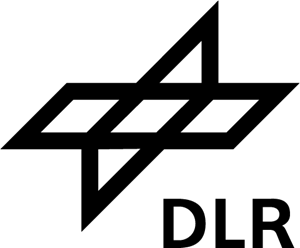
\includegraphics[width=0.2\textwidth]{fig/ch00_DLR_Logo_1.png}
	\end{minipage}

	\begin{minipage}[][][c]{0.48\textwidth}
		\begin{flushleft}
			\textsf{\small\\ [0.35cm]
		\workInstitution\\ [0.4cm]
		\workFakultaet}
		\end{flushleft}
	\end{minipage}
	\begin{minipage}[][][c]{0.48\textwidth}
		\begin{flushright}
			\textsf{\small
		\workCompany\\ [0.4cm]
		\workInstitut\\ [0.1cm]
%		\workLab\\ [0.1cm]
%		\workProf
		}
		\end{flushright}
	\end{minipage}
	
	\thispagestyle{empty}
	
	\vspace{3cm}
	
	\begin{center}
		\textsf{\textbf{\large{\workTyp}}}\\
		\vspace{1.5cm}
			\textsf{\textbf{\Huge{\workTitel}}}\\
		\vspace{3cm}
			\textsf{\textbf{\large{\workAutor}}}\\
			\textsf{\textbf{\large{Matr.Nr.: \workMatrikelnummer}}}\\
		\vspace{0,5cm}
			\textsf{\normalsize{\workStadtDatum}}
		\vspace{1.5cm}
	\end{center}
	
%	\begin{tabbing}
%		\textbf{Ausgegeben am:}\qquad \= \kill
%		\textsf{Referent:} \> 	\textsf{\workReferent}\\[0.2cm]
%		\textsf{Korreferent:} \> \textsf{\workKorreferent}\\[0.2cm]
%		%\textsf{Ausgegeben am:} \> \textsf{\workAusgabe}\\[0.2cm]
%		\textsf{Eingereicht am:} \> \textsf{\workAbgabe}\\
%	\end{tabbing}
\end{titlepage}
%\clearpage
%\newpage
%\thispagestyle{empty}
%\mbox{~}
%\clearpage
%\newpage
\newpage 
%\thispagestyle{empty}

%\ % The empty page


							% title page
\newpage \thispagestyle{empty}
\vspace*{19cm}
\begin{tabbing}
    \textbf{Ausgegeben am:}\qquad \= \kill
    \textsf{Erstprüfer:} \> 	\textsf{\workReferent}\\[0.2cm]
    \textsf{Zweitprüfer:} \> \textsf{\workKorreferent}\\[0.2cm]
    \textsf{Angemeldet am} \> \textsf{\workAusgabe}\\[0.2cm]
    \textsf{Eingereicht am:} \> \textsf{\workAbgabe}\\[0.2cm]
    \textsf{Kolloquium am:} \> \textsf{\workKolloqium}\\[0.2cm]
\end{tabbing}


% NUR bei Abschlussarbeiten ->...
\onehalfspacing
% !TeX encoding = utf8
% !TeX program = pdflatex
% !TeX spellcheck = de-DE
%\clearpage \thispagestyle{empty}
\chapter*{Danksagung}
Lorem ipsum dolor sit amet, consetetur sadipscing elitr, sed diam nonumy eirmod tempor invidunt ut labore et dolore magna aliquyam erat, sed diam voluptua. At vero eos et accusam et justo duo dolores et ea rebum. Stet clita kasd gubergren, no sea takimata sanctus est Lorem ipsum dolor sit amet. Lorem ipsum dolor sit amet, consetetur sadipscing elitr, sed diam nonumy eirmod tempor invidunt ut labore et dolore magna aliquyam erat, sed diam voluptua. At vero eos et accusam et justo duo dolores et ea rebum. Stet clita kasd gubergren, no sea takimata sanctus est Lorem ipsum dolor sit amet. Lorem ipsum dolor sit amet, consetetur sadipscing elitr, sed diam nonumy eirmod tempor invidunt ut labore et dolore magna aliquyam erat, sed diam voluptua. At vero eos et accusam et justo duo dolores et ea rebum. Stet clita kasd gubergren, no sea takimata sanctus est Lorem ipsum dolor sit amet.   

Duis autem vel eum iriure dolor in hendrerit in vulputate velit esse molestie consequat, vel illum dolore eu feugiat nulla facilisis at vero eros et accumsan et iusto odio dignissim qui blandit praesent luptatum zzril delenit augue duis dolore te feugait nulla facilisi. Lorem ipsum dolor sit amet,
\ % The empty page
\thispagestyle{empty}
\chapter*{Kurzfassung}
In dieser Arbeit wird eine modellprädiktive Regelung eingeführt, um die Luftaustrittstemperatur des Receivers am Solarturm in Jülich unter Berücksichtigung zukünftiger Wolkenbedingungen zu regeln.
Zu diesem Zweck wird auch die Modellbildung des Heliostatenfeldes und des Receivers des Solarturms vorgestellt.
Die Stellgrößen des Reglers sind der Luftmassenstrom im Receiver sowie drei Streuungsfaktoren, die jedem Heliostaten ihren individuellen Zielpunkt auf dem Receiver zuweisen.
Die Strategie der Zielpunktverteilung basiert auf dem von García et al. veröffentlichten Algorithmus mit Ventil-Analogie \cite{Garcia2} und wurde differenzierbar approximiert.
Zur Bewertung der Regelung wurde ein Referenzszenario aus der Literatur vorgestellt und verschiedene Wolkenszenarien definiert.
Die Güte der Regelung bemisst sich an der Abweichung der Luftaustrittstemperatur von der Referenztemperatur bei Nennlast.
Die Simulation der Regelstrecke zeigt, dass bei exakter Wolkenvorhersage des Nowcastings eine Verringerung dieser Temperaturabweichung von bis zu $\SI{86.4}{\percent}$ erreicht wird.
Der Exergieeintrag in den Folgeprozess ist je nach Lichtdurchlässigkeit der Wolken um bis zu $\SI{19.2}{\percent}$ größer als im Referenzszenario.
Besonders bei geringer Verschattungsintensität ist die Regelung dabei sehr effektiv.
Die Betriebssicherheit des Kraftwerkes wird maßgeblich durch die Oberflächentemperatur des Receivers beeinflusst.
Eine Analyse fehlerhafter Wolkenprognosen zeigt, dass die Sicherheit für Vorhersagen der Wolkengeschwindigkeit von $\geq\SI{-11}{\percent}$ und für Vorhersagen der Lichtdurchlässigkeit von $\geq\SI{-5}{\percent}$ des Realwertes durch die Regelung gewährleistet ist.
Prädiktionen schnellerer Wolken oder höherer Lichtdurchlässigkeiten als real auftretend stellen keine Gefahr für die Sicherheit des Kraftwerkes dar.
Auf Basis dieser Arbeit kann die Regelung durch zusätzliche Testszenarien und alternative Software verbessert und an der Realanlage getestet werden.

\chapter*{Abstract}
In this work, a model predictive control is introduced to control the air outlet temperature of the receiver at the solar tower in Jülich considering future cloud conditions.
For this purpose, the modeling of the heliostat field and the receiver of the solar tower is also presented.
The manipulated variables of the controller are the air mass flow in the receiver and three dispersion factors, which assign each heliostat its individual target point on the receiver.
The target point distribution strategy is based on the algorithm with valve analogy published by García et al \cite{Garcia2} and was differentially approximated.
To evaluate the control, a reference scenario from the literature was presented and different cloud scenarios were defined.
The quality of the control is measured by the deviation of the air outlet temperature from the reference temperature at nominal operation conditions.
The simulation of the controlled system shows that a reduction of this temperature deviation of up to $\SI{86.4}{\percent}$ is achieved with accurate cloud prediction of the nowcasting.
The exergy input to the downstream process is up to $\SI{19.2}{\percent}$ larger than in the reference scenario, depending on the light transmission of the clouds.
Especially at low shading intensity, the control is very effectiv.
The operational safety of the power plant is significantly influenced by the surface temperature of the receiver.
An analysis of erroneous cloud predictions shows that the safety is ensured by the control for cloud speed predictions of $\geq\SI{-11}{\percent}$ and for light transmittance predictions of $\geq\SI{-5}{\percent}$ of the real value.
Predictions of faster clouds or higher light transmittances than actually occur do not pose a threat to power plant safety.
Based on this work, the control can be improved by additional test scenarios and alternative software and can be tested on the real plant.

% Zusammenfassung
% ...<- für Projektberichte auskommentieren


%% list of contents
\doublespacing
\tableofcontents
\cleardoublepage

%% list of figures
\addcontentsline{toc}{chapter}{\bfseries Abbildungsverzeichnis}
\renewcommand{\listfigurename}{Abbildungsverzeichnis}
\listoffigures
\cleardoublepage

%% list of tables
\addcontentsline{toc}{chapter}{\bfseries Tabellenverzeichnis}
\listoftables
\cleardoublepage

%% Abkürzungsverzeichnis muss HÄNDISCH eingetragen werden
\singlespacing
\addcontentsline{toc}{chapter}{\bfseries Abkürzungsverzeichnis}
\listof{figure}{Abkürzungs- und Symbolverzeichnis}
\newcommand{\acrounit}[1]{
    \acroextra{
        \hspace{-21mm}\makebox[18mm][l]{\si[per=frac,fraction=nice]{#1}}
    }
}
\begin{acronym}[LONGEST]
    %\acro{KÜRZEL}[ABKÜRZUNG]\quad{\acroextra{\makebox[22mm][l]{\si{ EINHEIT }}}BESCHREIBUNG}
    \large{\acro{Abk}[Abkürzung]~{\acroextra{\makebox[22mm][l]{\si{ \textbf{Einheit} }}}\textbf{Beschreibung}}}
    % \normalsize{
    %     \acro{Abc}[Abc]\quad{\acroextra{\makebox[22mm][l]{\si{ $^\circ$ }}}Alphabet}
    %     \acro{Bcd}[Bcd]\quad{\acroextra{\makebox[22mm][l]{\si{ $B_{cd}$ }}}Test}


    % }
\end{acronym}
\cleardoublepage


%Formelverzeichnis
\doublespacing
\addcontentsline{toc}{chapter}{\bfseries Formelverzeichnis}
\newcommand{\listequationsname}{Formelverzeichnis}
\newlistof{myequations}{equ}{\listequationsname}
\newcommand{\myequations}[1]{%
    \addcontentsline{equ}{myequations}{\protect\numberline{\theequation}#1}\par}

\listofmyequations

\cleardoublepage




% ========================= CONTENT ========================
% ==========================================================
\newpage
\onehalfspacing

\newcounter{savepage}                                                   % Fortlaufende Nummerierung der Seiten
\setcounter{savepage}{\number\value{page}}                              % Fortlaufende Nummerierung der Seiten

\pagenumbering{arabic}                                                  % arabic page numbering
\setcounter{page}{1}
%\setcounter{page}{\number\value{savepage}}								% Fortlaufende Nummerierung der Seiten

\chapter{Einleitung} \label{ch_Einleitung}
Paar einleitende Worte.
Hier auch schreiben, dass die Abbildungen in englischer Sprache sind und die Texte in Deutsch.


\section{Motivation} \label{sec_Motivation}
Motivation, siehe Davids Masterarbeit, siehe Gall Diss.

\section{Zielsetzung} \label{sec_Zielsetzung}
Zielsetzung, siehe Zielsetzung an Kim und auf Bachelorarbeit Einreichung.
Außerdem siehe David Ziele was die Simulationen angeht:
\begin{itemize}
    \item Wie viel besser ist der MPC, wenn er von den Wolken weiß?
    \item Wo sind zu jedem Szenario die Grenzen? Also wie viel \% darf die MPC Vorhersage vor der eigentlichen Simulation abweichen?
\end{itemize}
Außerdem hat David schon hier seine Quelle drin, wie man einen Controller auslegt.
Wohin mit diesem Inhalt?

\section{Struktur der Arbeit} \label{sec_Struktur}
Hier die Struktur hin.


\chapter{Stand der Technik}\label{ch_StandTechnik}
\section{Erstes Unterkapitel}



\subsection{Erstes Unter- Unterkapitel}


\newpage
\emptywithpagenumber % include chapter
\chapter{Drittes Kapitel}\label{ch_StandTechnik}
Lorem ipsum dolor sit amet, consetetur sadipscing elitr, sed diam nonumy eirmod tempor invidunt ut labore et dolore magna aliquyam erat, sed diam voluptua. At vero eos et accusam et justo duo dolores et ea rebum. Stet clita kasd gubergren, no sea takimata sanctus est Lorem ipsum dolor sit amet. Lorem ipsum dolor sit amet, consetetur sadipscing elitr, sed diam nonumy eirmod tempor invidunt ut labore et dolore magna aliquyam erat, sed diam voluptua. At vero eos et accusam et justo duo dolores et ea rebum. Stet clita kasd gubergren, no sea takimata sanctus est Lorem ipsum dolor sit amet. Lorem ipsum dolor sit amet, consetetur sadipscing elitr, sed diam nonumy eirmod tempor invidunt ut labore et dolore magna aliquyam erat, sed diam voluptua. At vero eos et accusam et justo duo dolores et ea rebum. Stet clita kasd gubergren, no sea takimata sanctus est Lorem ipsum dolor sit amet.

Duis autem vel eum iriure dolor in hendrerit in vulputate velit esse molestie consequat, vel illum dolore eu feugiat nulla facilisis at vero eros et accumsan et iusto odio dignissim qui blandit praesent luptatum zzril delenit augue duis dolore te feugait nulla facilisi.

Hier kommt auf jeden Fall ein Zitat rein \cite{Follinger.2016}. \cite{ifmelectronic.2004}


% ========================= APPENDIX =========================
% ============================================================
\cleardoublepage
\setcounter{savepage}{\number\value{page}}                              % Fortlaufende Nummerierung der Seiten
\pagenumbering{Roman}                                                   % roman page numbering
\setcounter{page}{\number\value{savepage}}								% Fortlaufende Nummerierung	der Seiten	

% \printbibliography[											% print bibliography
%     heading = bibintoc,											% add to toc
%     title={Literaturverzeichnis}
% ]
% \bibliographystyle{plain}
% \bibliography{ch/bibliography}

\addcontentsline{toc}{chapter}{\bfseries Literaturverzeichnis}
\bibliographystyle{ieeetr}
\bibliography{ch/bibliography}
% Ich Sobald ich auf
% \bibliographystyle{maas}
% gewechselt habe, aktualisiert sich das Verzeichnis nicht mehr. Dann muss einmalig der \bibliography{} Befehl auskommentiert werden und das Verzeichnis kann neu kompiliert werden.
% Klappt leider noch nicht.
% Wenn alles auskommentiert ist kann ich die Quellen mit \cite{} normal schreiben und das aktualisiert dann auch, der obige Teil wenn die Kapitel einkommentiert sind macht aber leider nix.

\cleardoublepage

\appendix
\chapter{Anhang}\label{ch_anhang}
\begin{figure}[h!]
    \centering
    \setlength{\fboxsep}{1pt}
    \setlength{\fboxrule}{1pt}
    \fbox{\includegraphics[width=0.92\textwidth]{C:/Users/gesc_ma/VSCode MPC Projekt/dynaovrcontroller/dynaovrcontroller/aimpoint_control_scenarios/plots/00_no_control/shading_120sec_75_30mps.png}}
    \caption[Simulationsverlauf für das Cloud Standby Referenzszenario bei Verschattung um $\SI{25}{\percent}$ und $\SI{30}{\metre\per\second}$ Wolkengeschwindigkeit]{Simulationsverlauf für das Cloud Standby Referenzszenario bei Verschattung um $\SI{25}{\percent}$ und $\SI{30}{\metre\per\second}$ Wolkengeschwindigkeit}
    \label{fig_nocontrol7530}
\end{figure}

\begin{figure}[h!]
    \centering
    \setlength{\fboxsep}{1pt}
    \setlength{\fboxrule}{1pt}
    \fbox{\includegraphics[width=0.92\textwidth]{C:/Users/gesc_ma/VSCode MPC Projekt/dynaovrcontroller/dynaovrcontroller/aimpoint_control_scenarios/plots/01_mpc_all_information/shading_120sec_75_30mps.png}}
    \caption[Simulationsverlauf für den Betrieb mit abweichungsfreier Einstrahlungsvorhersage bei Verschattung um $\SI{25}{\percent}$ und $\SI{30}{\metre\per\second}$ Wolkengeschwindigkeit]{Simulationsverlauf für den Betrieb mit abweichungsfreier Einstrahlungsvorhersage bei Verschattung um $\SI{25}{\percent}$ und $\SI{30}{\metre\per\second}$ Wolkengeschwindigkeit}
    \label{fig_allwissend7530}
\end{figure}

\begin{figure}[h!]
    \centering
    \setlength{\fboxsep}{1pt}
    \setlength{\fboxrule}{1pt}
    \fbox{\includegraphics[width=0.99\textwidth]{C:/Users/gesc_ma/VSCode MPC Projekt/dynaovrcontroller/dynaovrcontroller/aimpoint_control_scenarios/plots/00_no_control/shading_120sec_00_30mps.png}}
    \caption[Simulationsverlauf für das Cloud Standby Referenzszenario bei Verschattung um $\SI{100}{\percent}$ und $\SI{30}{\metre\per\second}$ Wolkengeschwindigkeit]{Simulationsverlauf für das Cloud Standby Referenzszenario bei Verschattung um $\SI{100}{\percent}$ und $\SI{30}{\metre\per\second}$ Wolkengeschwindigkeit}
    \label{fig_cloudstandby0030}
\end{figure}

\begin{figure}[h!]
    \centering
    \setlength{\fboxsep}{1pt}
    \setlength{\fboxrule}{1pt}
    \fbox{\includegraphics[width=0.99\textwidth]{C:/Users/gesc_ma/VSCode MPC Projekt/dynaovrcontroller/dynaovrcontroller/aimpoint_control_scenarios/plots/01_mpc_all_information/shading_120sec_00_30mps.png}}
    \caption[Simulationsverlauf für den Betrieb mit abweichungsfreier Einstrahlungsvorhersage bei Verschattung um $\SI{100}{\percent}$ und $\SI{30}{\metre\per\second}$ Wolkengeschwindigkeit]{Simulationsverlauf für den Betrieb mit abweichungsfreier Einstrahlungsvorhersage bei Verschattung um $\SI{100}{\percent}$ und $\SI{30}{\metre\per\second}$ Wolkengeschwindigkeit}
    \label{fig_allwissend0030}
\end{figure}

\begin{figure}[h!]
    \centering
    \setlength{\fboxsep}{1pt}
    \setlength{\fboxrule}{1pt}
    \fbox{\includegraphics[width=0.99\textwidth]{C:/Users/gesc_ma/VSCode MPC Projekt/dynaovrcontroller/dynaovrcontroller/aimpoint_control_scenarios/plots/02_mpc_thinking_clearsky/shading_120sec_75_20mps.png}}
    \caption[Simulationsverlauf für den Betrieb ohne Einstrahlungsvorhersage bei Lichtdurchlässigkeit der Wolke von $\SI{75}{\percent}$ und $\SI{20}{\metre\per\second}$ Wolkengeschwindigkeit]{Simulationsverlauf für den Betrieb ohne Einstrahlungsvorhersage bei Lichtdurchlässigkeit der Wolke von $\SI{75}{\percent}$ und $\SI{20}{\metre\per\second}$ Wolkengeschwindigkeit}
    \label{fig_unwissend7520}
\end{figure}

\begin{figure}[h!]
    \centering
    \setlength{\fboxsep}{1pt}
    \setlength{\fboxrule}{1pt}
    \fbox{\includegraphics[width=0.99\textwidth]{C:/Users/gesc_ma/VSCode MPC Projekt/dynaovrcontroller/dynaovrcontroller/aimpoint_control_scenarios/plots/01_mpc_all_information/shading_120sec_75_20mps.png}}
    \caption[Simulationsverlauf für den Betrieb mit abweichungsfreier Einstrahlungsvorhersage bei Lichtdurchlässigkeit der Wolke von $\SI{75}{\percent}$ und $\SI{20}{\metre\per\second}$ Wolkengeschwindigkeit]{Simulationsverlauf für den Betrieb mit abweichungsfreier Einstrahlungsvorhersage bei Lichtdurchlässigkeit der Wolke von $\SI{75}{\percent}$ und $\SI{20}{\metre\per\second}$ Wolkengeschwindigkeit}
    \label{fig_allwissend7520}
\end{figure}

\begin{figure}[h!]
    \centering
    \setlength{\fboxsep}{1pt}
    \setlength{\fboxrule}{1pt}
    \fbox{\includegraphics[width=0.99\textwidth]{C:/Users/gesc_ma/VSCode MPC Projekt/dynaovrcontroller/dynaovrcontroller/aimpoint_control_scenarios/plots/02_mpc_thinking_clearsky/shading_120sec_00_20mps.png}}
    \caption[Simulationsverlauf für den Betrieb ohne Einstrahlungsvorhersage bei Verschattung von $\SI{100}{\percent}$ und $\SI{20}{\metre\per\second}$ Wolkengeschwindigkeit]{Simulationsverlauf für den Betrieb ohne Einstrahlungsvorhersage bei Verschattung von $\SI{100}{\percent}$ und $\SI{20}{\metre\per\second}$ Wolkengeschwindigkeit}
    \label{fig_unwissend0020}
\end{figure}

\begin{figure}[h!]
    \centering
    \setlength{\fboxsep}{1pt}
    \setlength{\fboxrule}{1pt}
    \fbox{\includegraphics[width=0.99\textwidth]{C:/Users/gesc_ma/VSCode MPC Projekt/dynaovrcontroller/dynaovrcontroller/aimpoint_control_scenarios/plots/01_mpc_all_information/shading_120sec_00_20mps.png}}
    \caption[Simulationsverlauf für den Betrieb mit abweichungsfreier Einstrahlungsvorhersage bei Verschattung von $\SI{100}{\percent}$ und $\SI{20}{\metre\per\second}$ Wolkengeschwindigkeit]{Simulationsverlauf für den Betrieb mit abweichungsfreier Einstrahlungsvorhersage bei Verschattung von $\SI{100}{\percent}$ und $\SI{20}{\metre\per\second}$ Wolkengeschwindigkeit}
    \label{fig_allwissend0020}
\end{figure}

\begin{figure}[h!]
    \centering
    \setlength{\fboxsep}{1pt}
    \setlength{\fboxrule}{1pt}
    \fbox{\includegraphics[width=0.99\textwidth]{C:/Users/gesc_ma/VSCode MPC Projekt/dynaovrcontroller/dynaovrcontroller/aimpoint_control_scenarios/plots/00_no_control/shading_120sec_75_20mps.png}}
    \caption[Simulationsverlauf für das Cloud Standby Referenzszenario bei Lichtdurchlässigkeit von um $\SI{25}{\percent}$ und $\SI{20}{\metre\per\second}$ Wolkengeschwindigkeit]{Simulationsverlauf für das Cloud Standby Referenzszenario bei Lichtdurchlässigkeit von um $\SI{25}{\percent}$ und $\SI{20}{\metre\per\second}$ Wolkengeschwindigkeit}
    \label{fig_cloudstandby7520}
\end{figure}

\begin{figure}[h!]
    \centering
    \setlength{\fboxsep}{1pt}
    \setlength{\fboxrule}{1pt}
    \fbox{\includegraphics[width=0.99\textwidth]{C:/Users/gesc_ma/VSCode MPC Projekt/dynaovrcontroller/dynaovrcontroller/aimpoint_control_scenarios/plots/00_no_control/shading_120sec_00_20mps.png}}
    \caption[Simulationsverlauf für das Cloud Standby Referenzszenario bei Verschattung um $\SI{100}{\percent}$ und $\SI{20}{\metre\per\second}$ Wolkengeschwindigkeit]{Simulationsverlauf für das Cloud Standby Referenzszenario bei Verschattung um $\SI{100}{\percent}$ und $\SI{20}{\metre\per\second}$ Wolkengeschwindigkeit}
    \label{fig_cloudstandby0020}
\end{figure}

\begin{figure}[h!]
    \centering
    \setlength{\fboxsep}{1pt}
    \setlength{\fboxrule}{1pt}
    \fbox{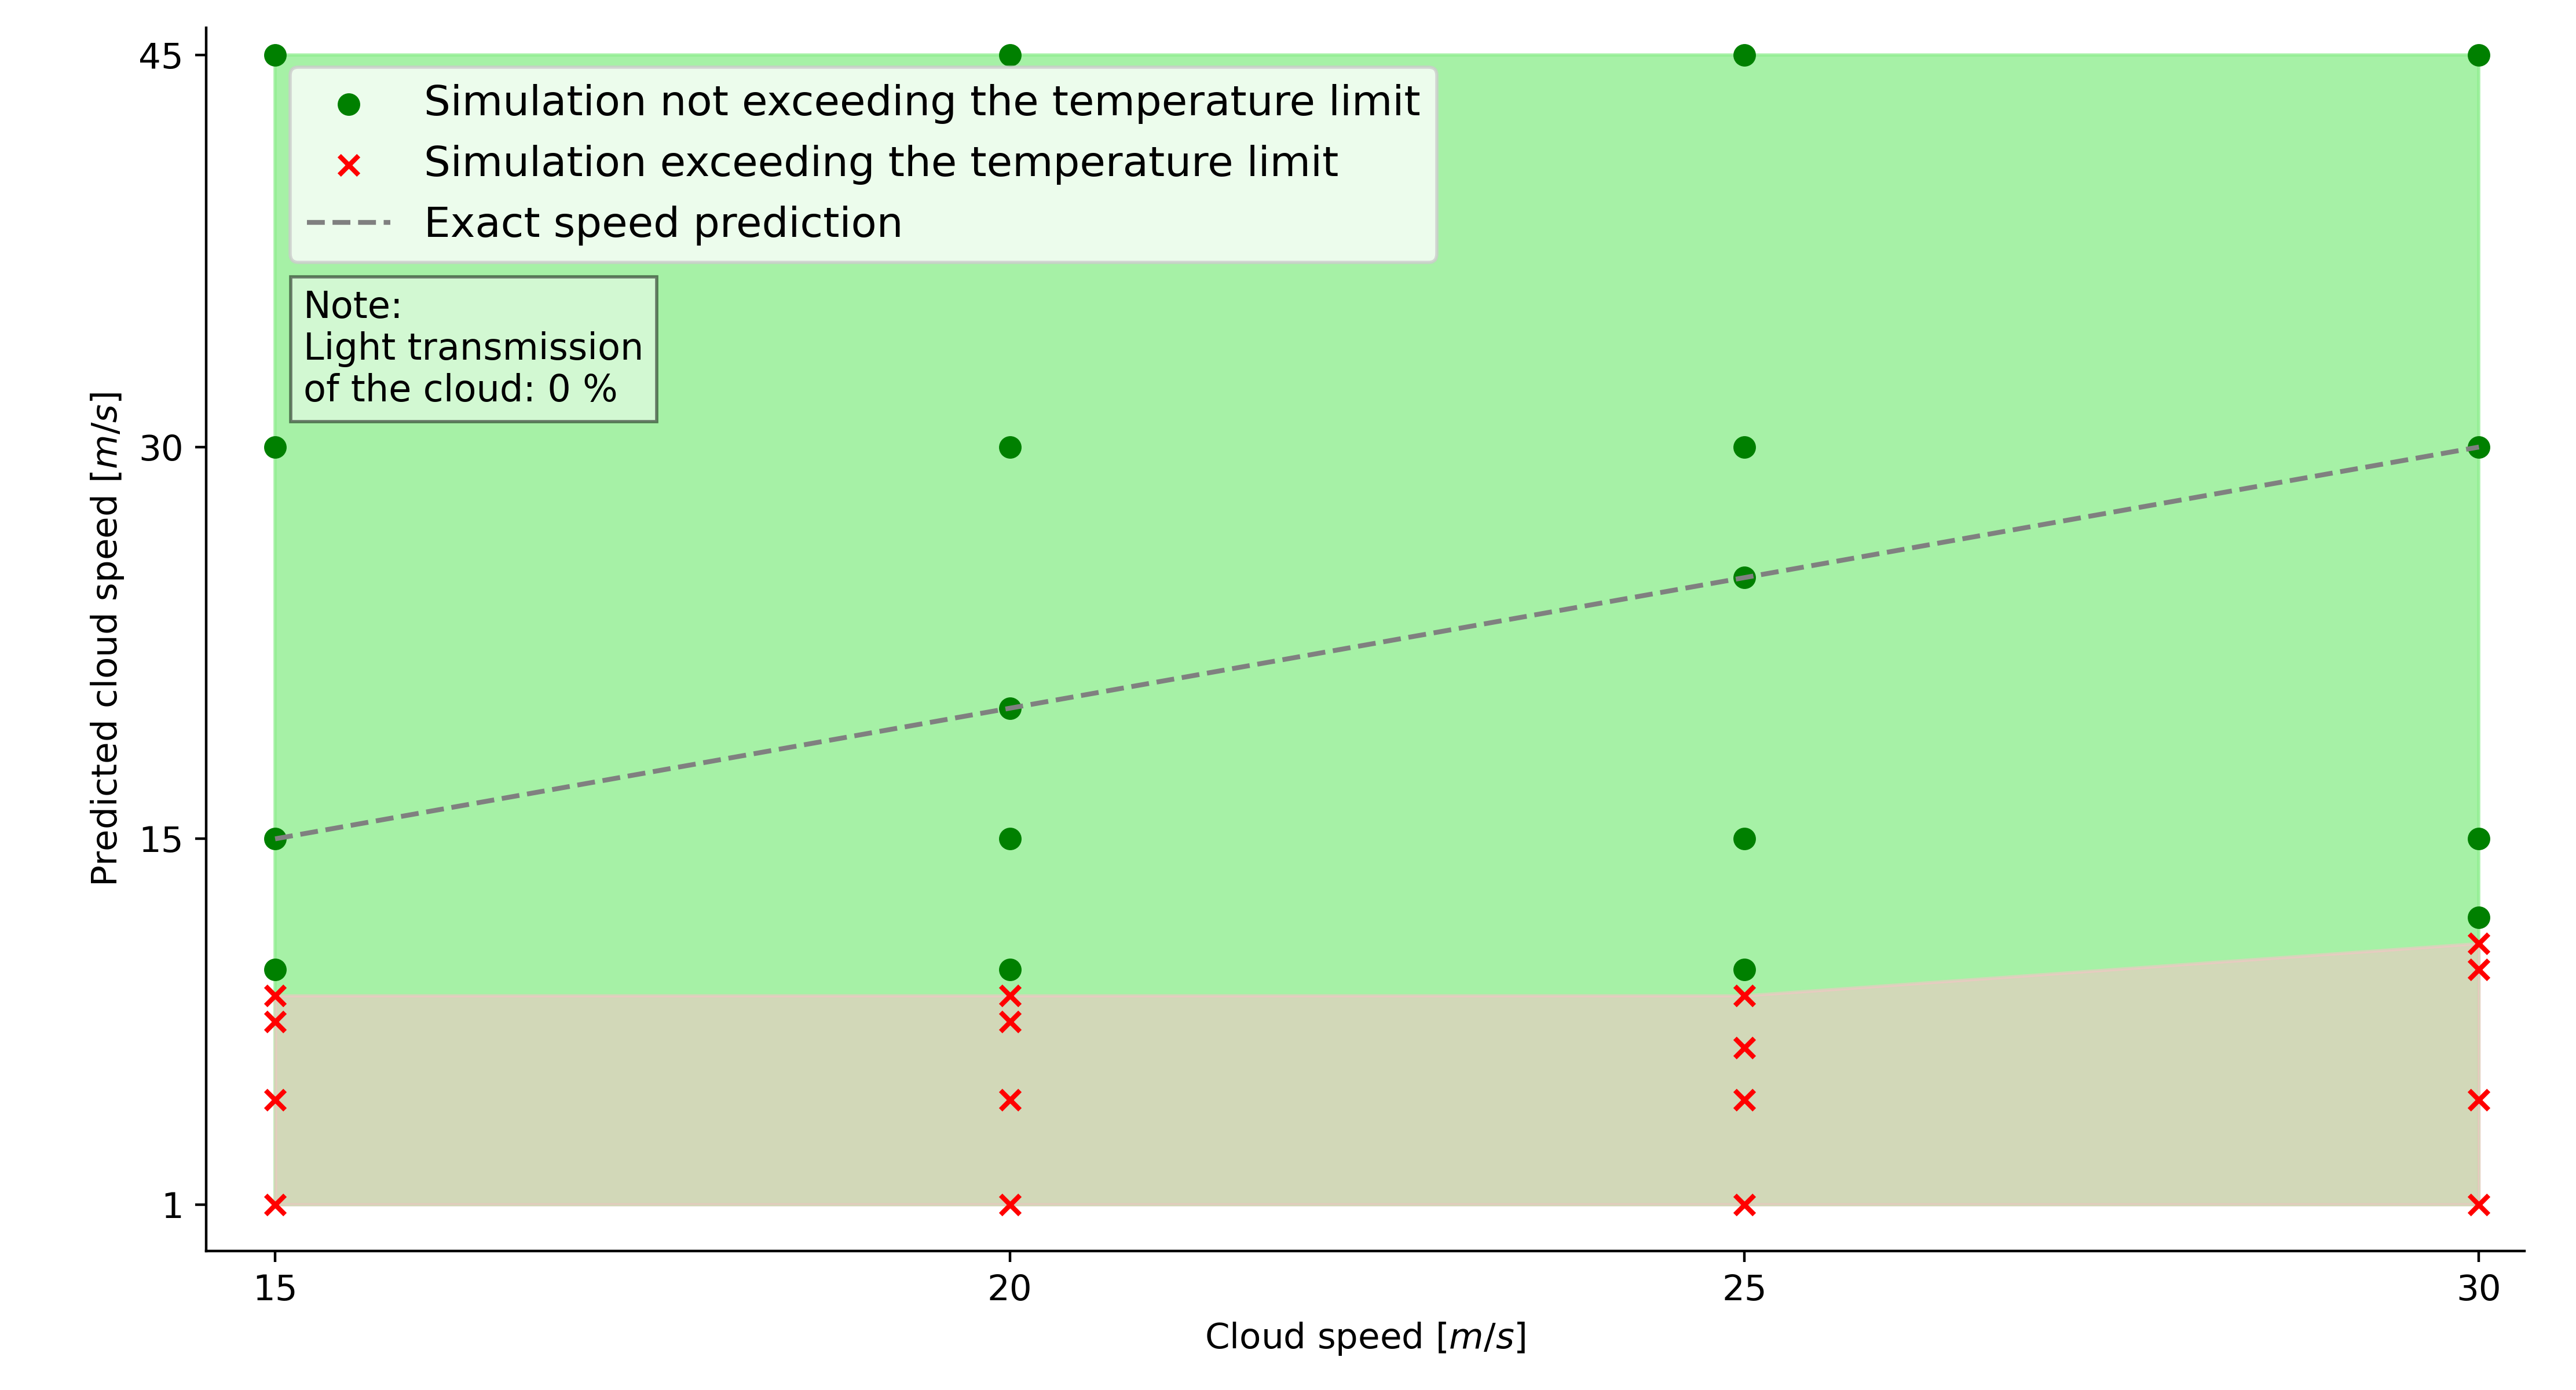
\includegraphics[width=0.99\textwidth]{C:/Users/gesc_ma/VSCode MPC Projekt/dynaovrcontroller/dynaovrcontroller/aimpoint_control_scenarios/plots/21_analyze_speed_uncertainty/safe_simulations_shading_0.png}}
    \caption[Analyse der erlaubten Abweichung in der Prädiktion der Wolkengeschwindigkeit für die Lichtdurchlässigkeit von $\SI{0}{\percent}$]{Analyse der erlaubten Abweichung in der Prädiktion der Wolkengeschwindigkeit für die Lichtdurchlässigkeit von $\SI{0}{\percent}$}
    \label{fig_speed00}
\end{figure}

\begin{figure}[h!]
    \centering
    \setlength{\fboxsep}{1pt}
    \setlength{\fboxrule}{1pt}
    \fbox{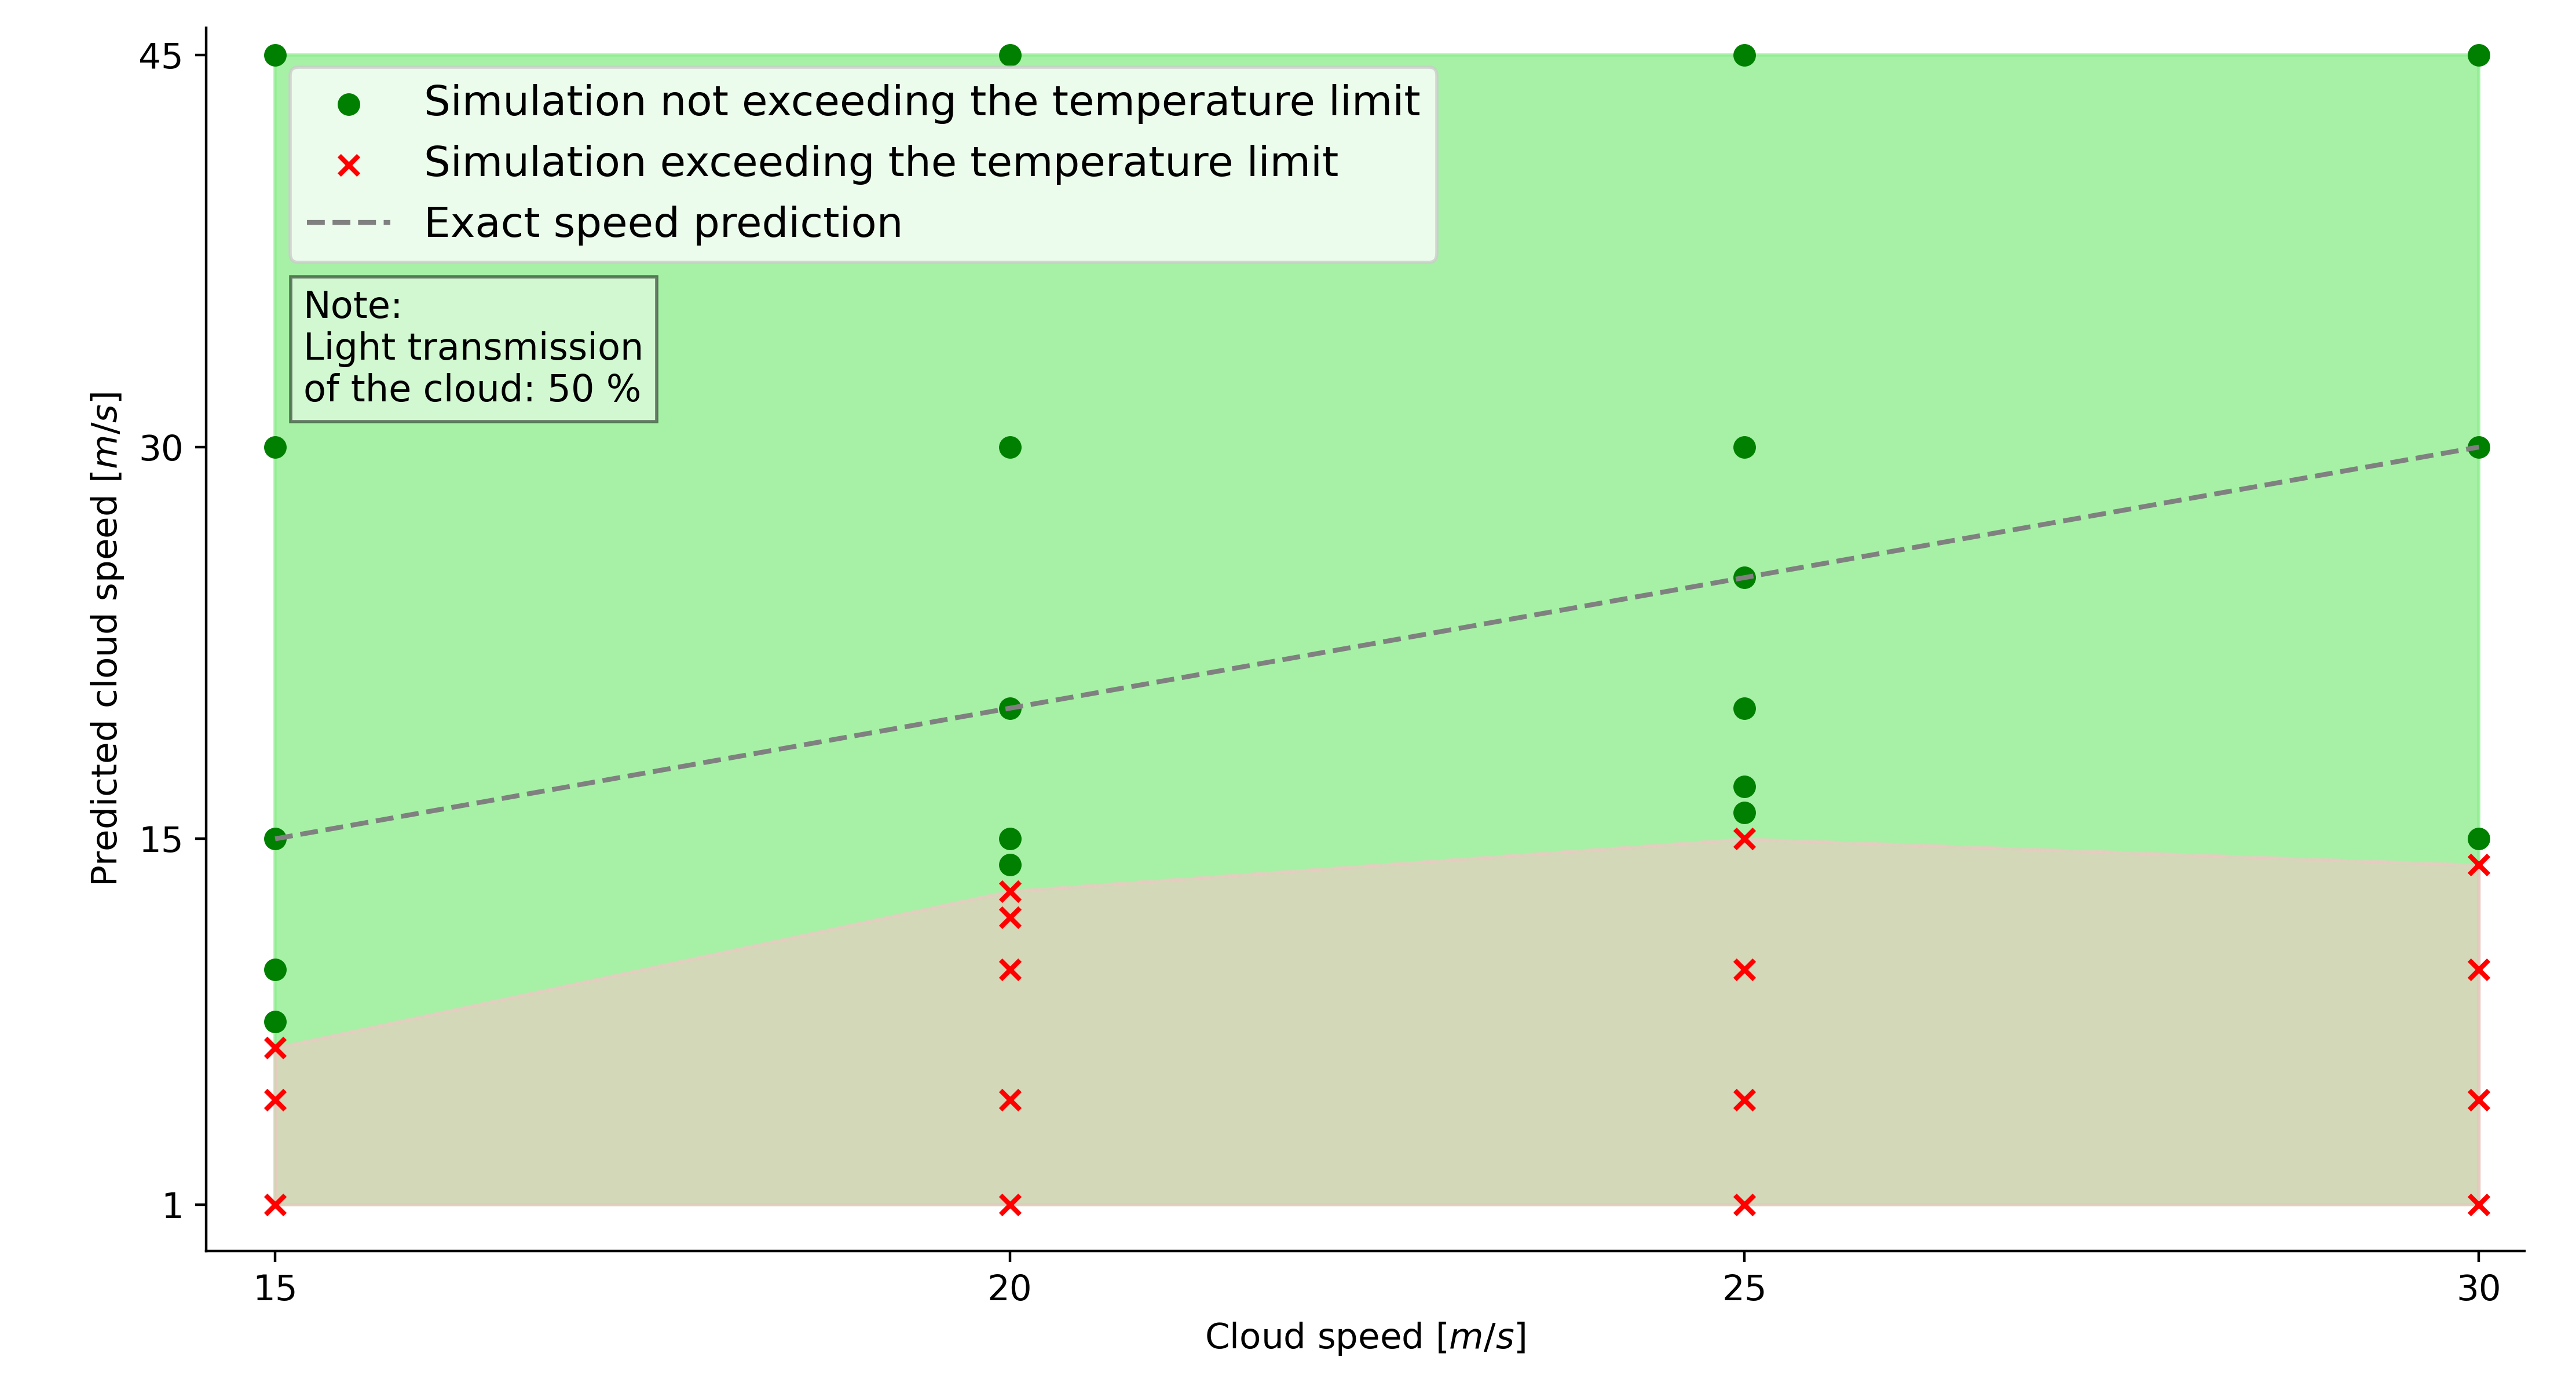
\includegraphics[width=0.99\textwidth]{C:/Users/gesc_ma/VSCode MPC Projekt/dynaovrcontroller/dynaovrcontroller/aimpoint_control_scenarios/plots/21_analyze_speed_uncertainty/safe_simulations_shading_50.png}}
    \caption[Analyse der erlaubten Abweichung in der Prädiktion der Wolkengeschwindigkeit für die Lichtdurchlässigkeit von $\SI{50}{\percent}$]{Analyse der erlaubten Abweichung in der Prädiktion der Wolkengeschwindigkeit für die Lichtdurchlässigkeit von $\SI{50}{\percent}$}
    \label{fig_speed50}
\end{figure}

\begin{figure}[h!]
    \centering
    \setlength{\fboxsep}{1pt}
    \setlength{\fboxrule}{1pt}
    \fbox{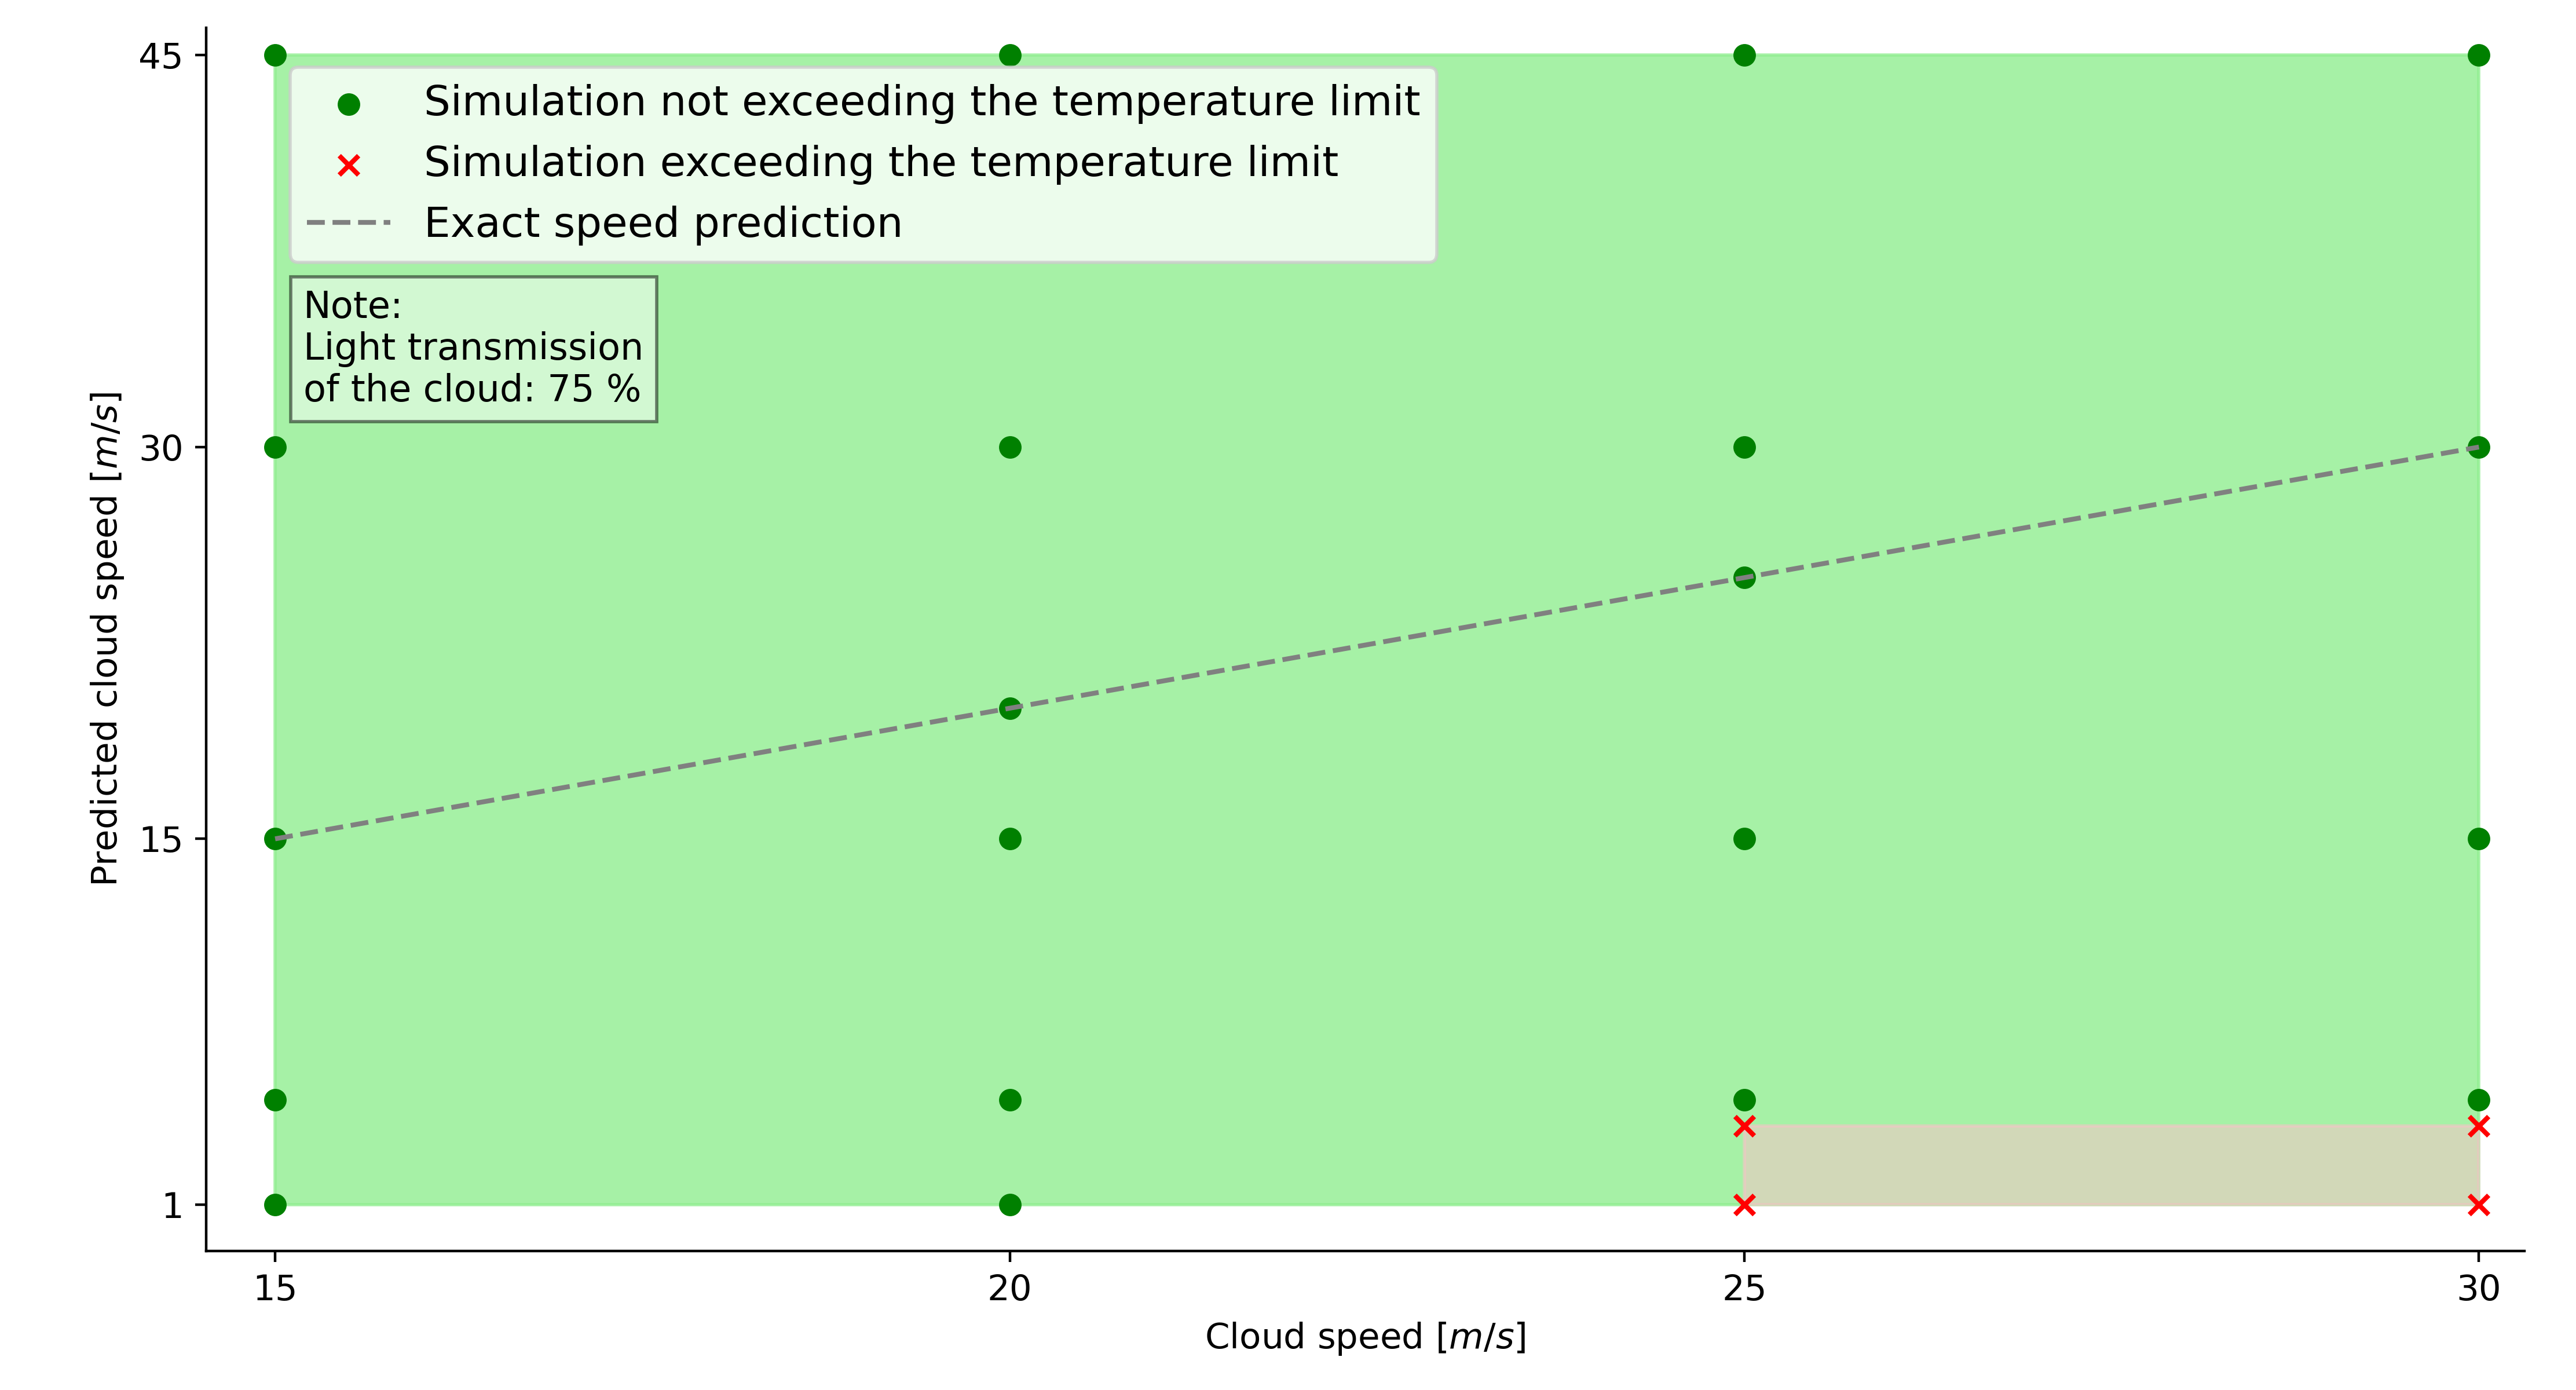
\includegraphics[width=0.99\textwidth]{C:/Users/gesc_ma/VSCode MPC Projekt/dynaovrcontroller/dynaovrcontroller/aimpoint_control_scenarios/plots/21_analyze_speed_uncertainty/safe_simulations_shading_75.png}}
    \caption[Analyse der erlaubten Abweichung in der Prädiktion der Wolkengeschwindigkeit für die Lichtdurchlässigkeit von $\SI{75}{\percent}$]{Analyse der erlaubten Abweichung in der Prädiktion der Wolkengeschwindigkeit für die Lichtdurchlässigkeit von $\SI{75}{\percent}$}
    \label{fig_speed75}
\end{figure}

\begin{figure}[h!]
    \centering
\setlength{\fboxsep}{1pt}
\setlength{\fboxrule}{1pt}
\fbox{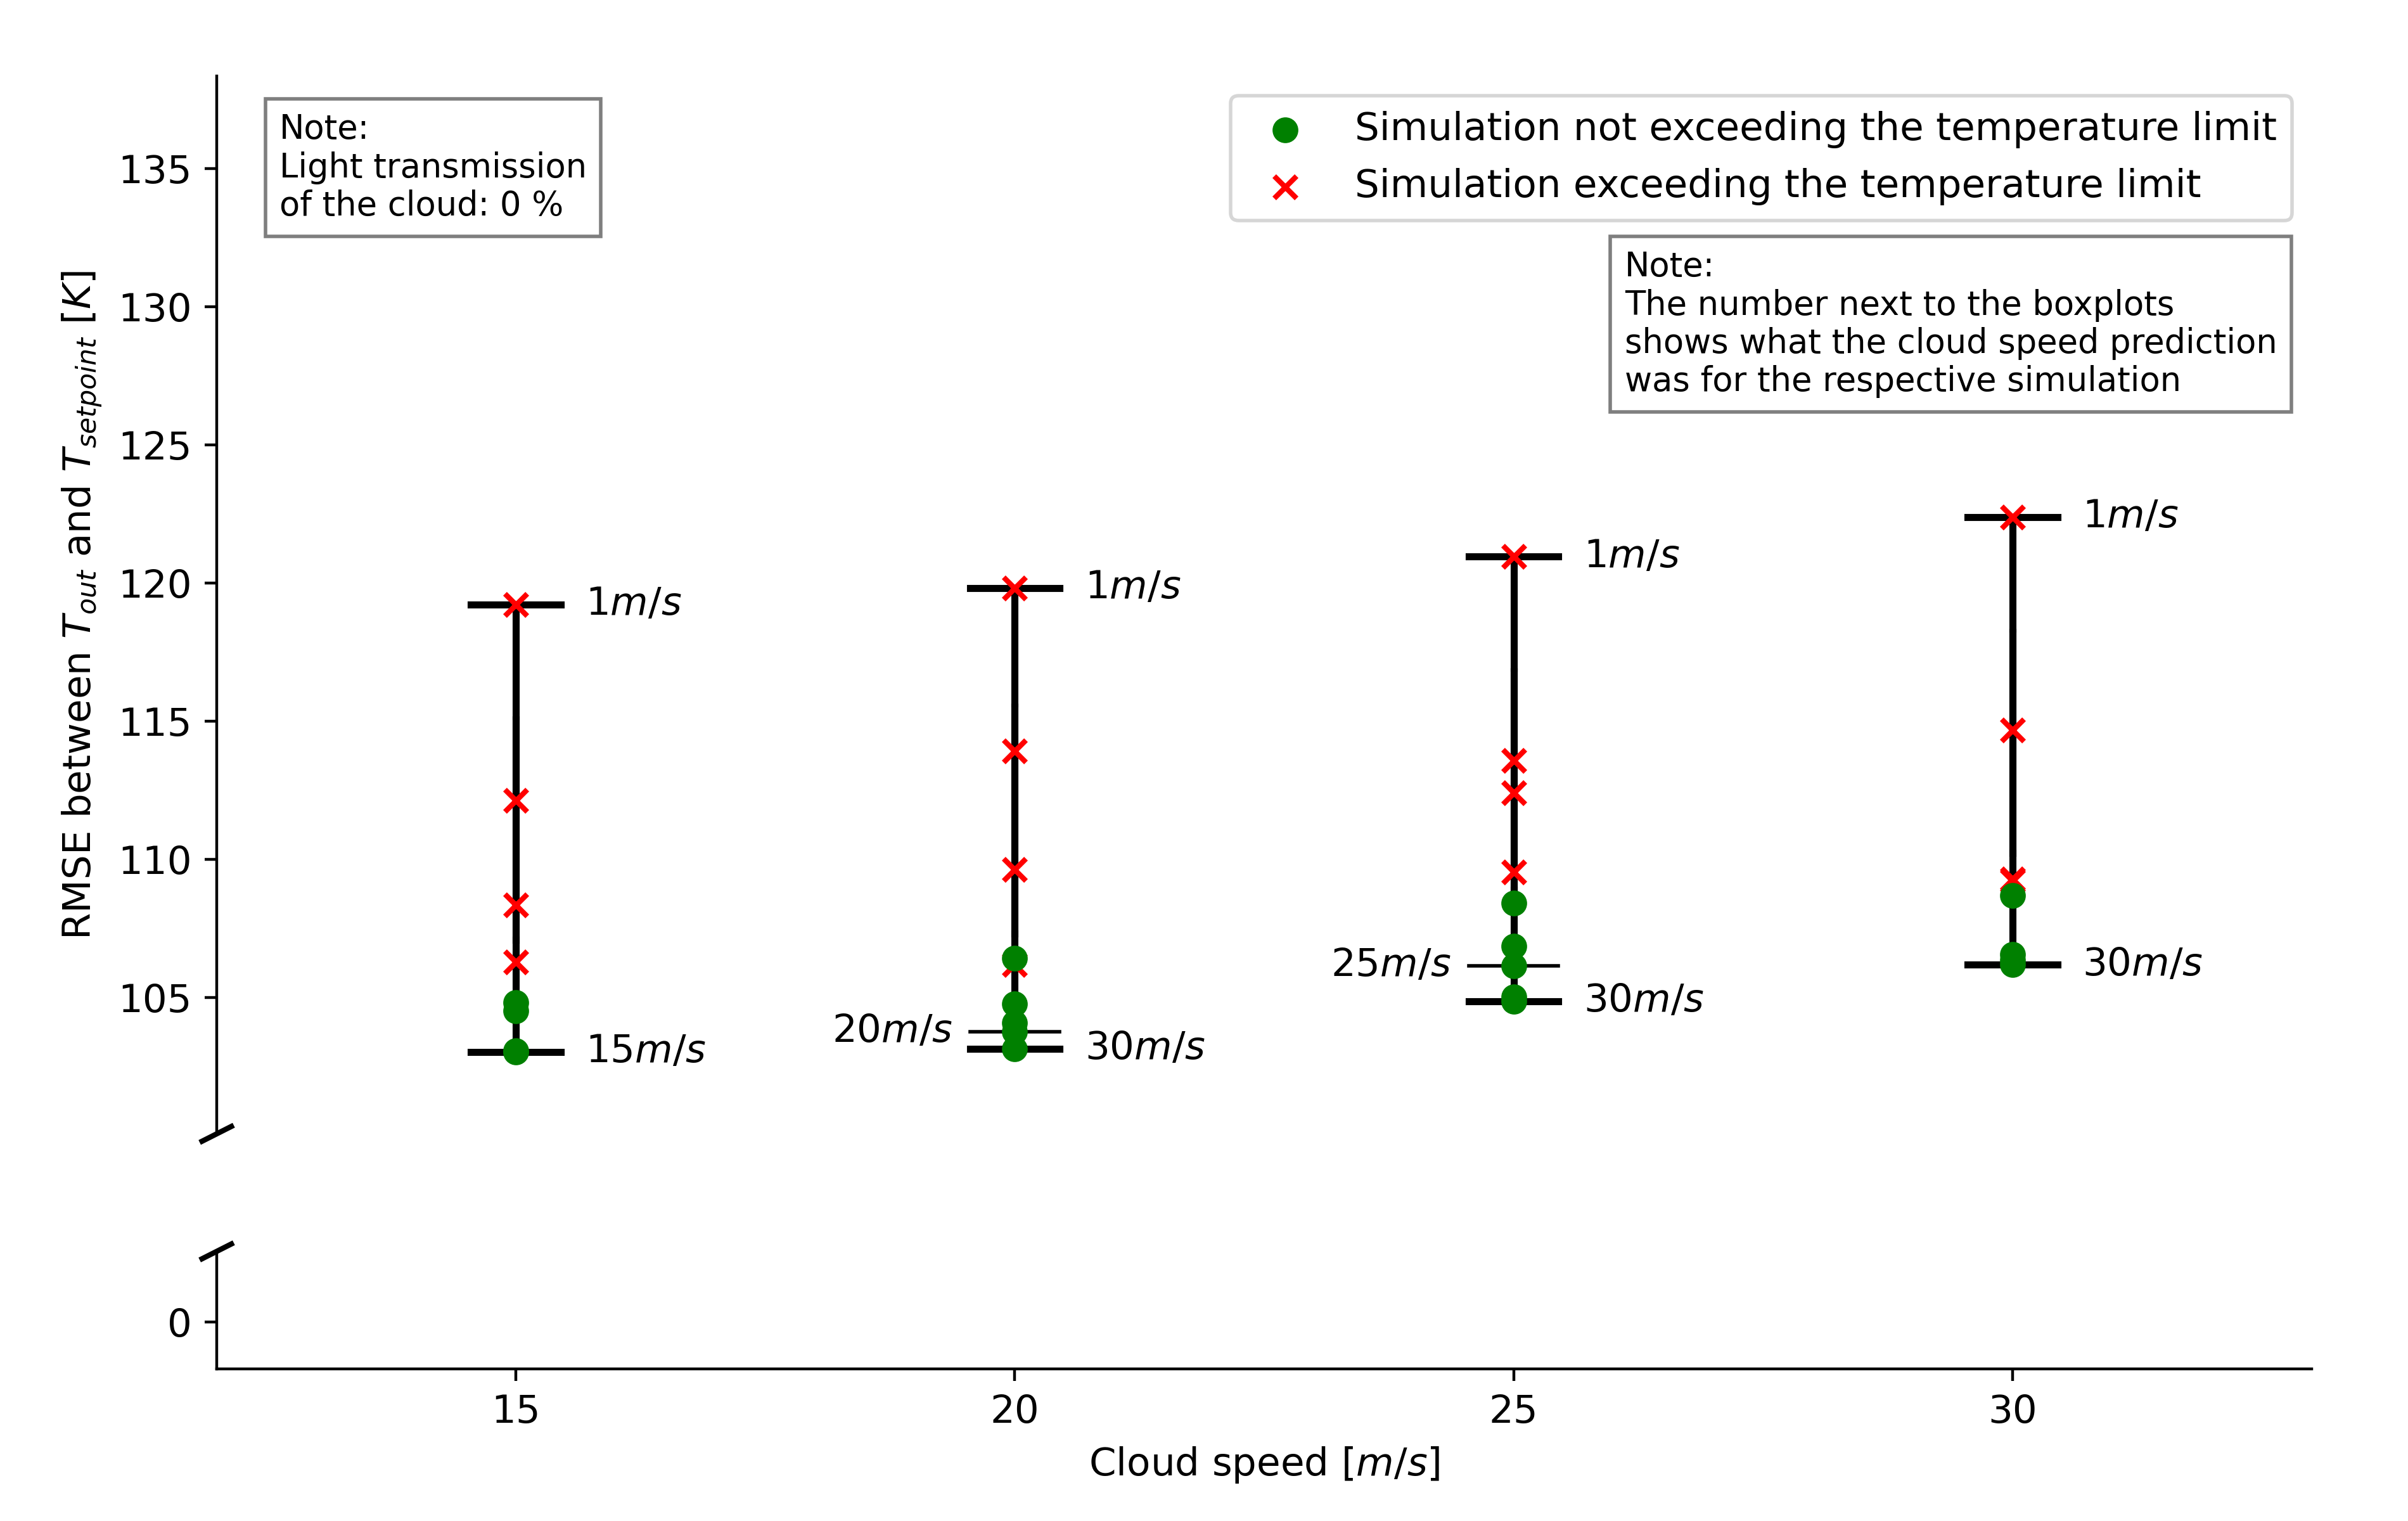
\includegraphics[width=0.99\textwidth]{C:/Users/gesc_ma/VSCode MPC Projekt/dynaovrcontroller/dynaovrcontroller/aimpoint_control_scenarios/plots/21_analyze_speed_uncertainty/rmse_per_speed_shading_0.png}}
\caption[Analyse des RMSE für unterschiedliche Prädiktionen der Wolkengeschwindigkeiten für eine Lichtdurchlässigkeit der Wolke von $\SI{0}{\percent}$]{Analyse des RMSE für unterschiedliche Prädiktionen der Wolkengeschwindigkeiten für eine Lichtdurchlässigkeit der Wolke von $\SI{0}{\percent}$}
\label{fig_speed00RMSE}
\end{figure}

\begin{figure}[h!]
    \centering
\setlength{\fboxsep}{1pt}
\setlength{\fboxrule}{1pt}
\fbox{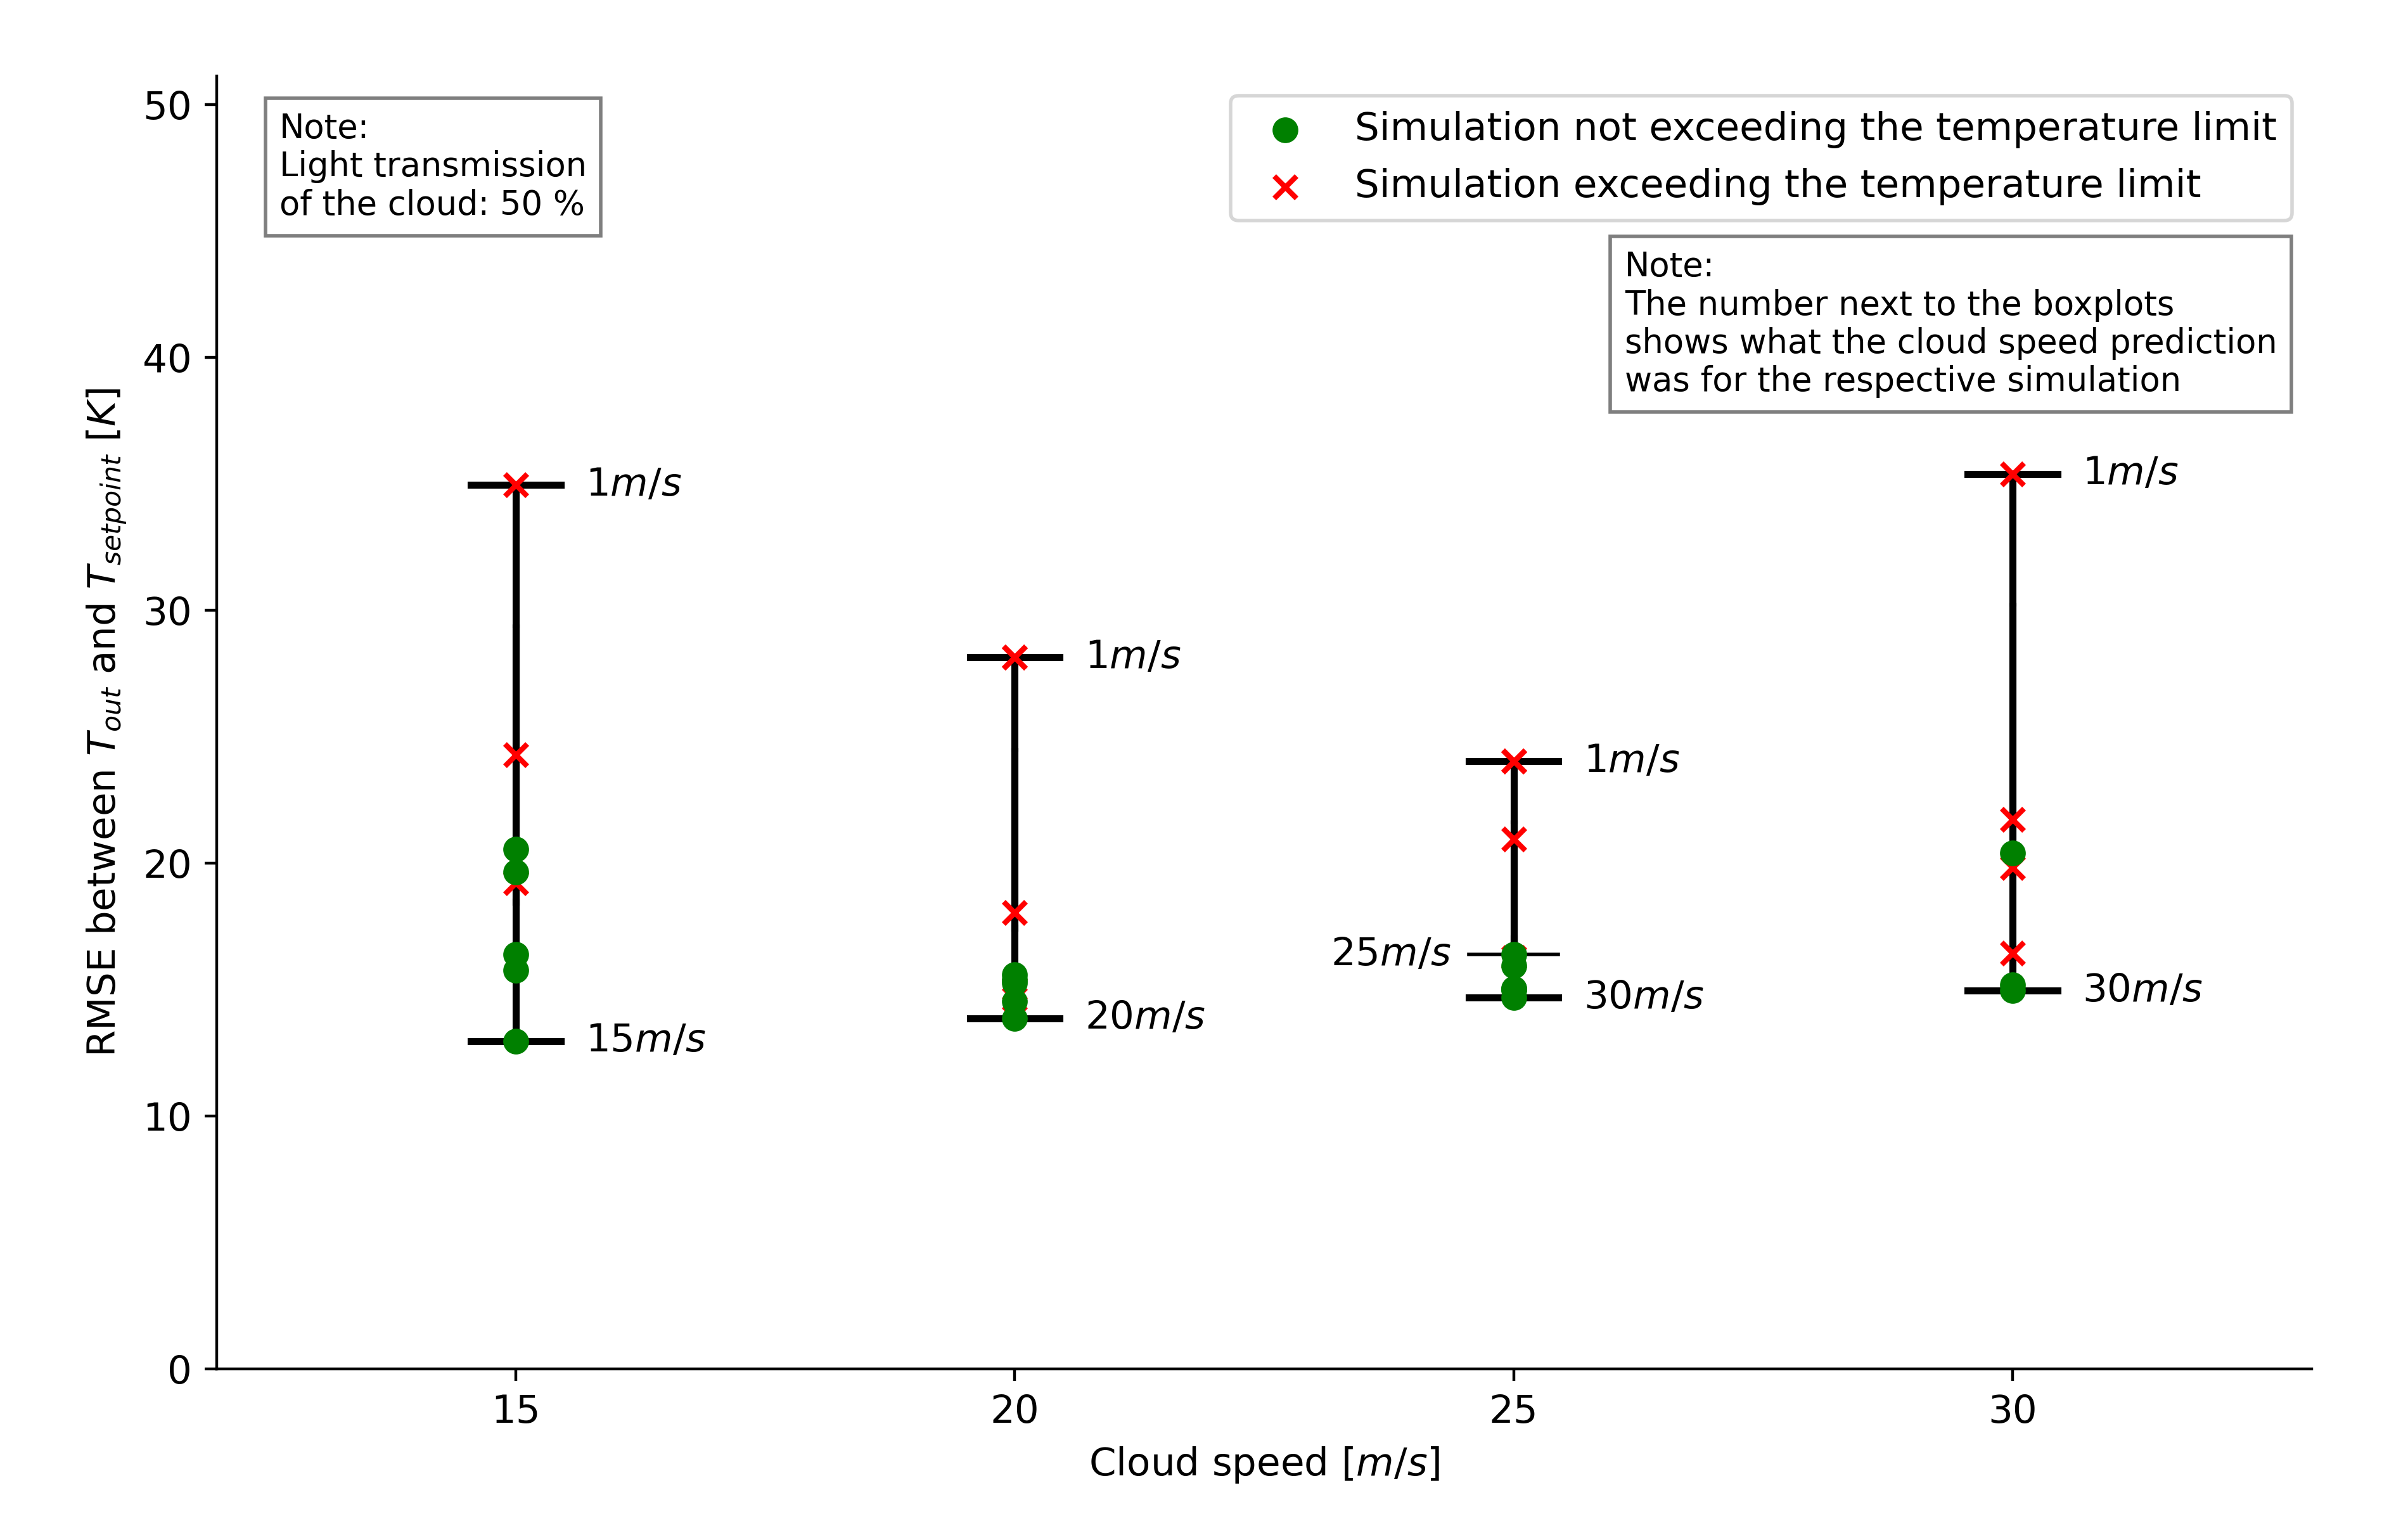
\includegraphics[width=0.89\textwidth]{C:/Users/gesc_ma/VSCode MPC Projekt/dynaovrcontroller/dynaovrcontroller/aimpoint_control_scenarios/plots/21_analyze_speed_uncertainty/rmse_per_speed_shading_50.png}}
\caption[Analyse des RMSE für unterschiedliche Prädiktionen der Wolkengeschwindigkeiten für eine Lichtdurchlässigkeit der Wolke von $\SI{50}{\percent}$]{Analyse des RMSE für unterschiedliche Prädiktionen der Wolkengeschwindigkeiten für eine Lichtdurchlässigkeit der Wolke von $\SI{50}{\percent}$}
\label{fig_speed50RMSE}
\end{figure}

\begin{figure}[h!]
    \centering
    \setlength{\fboxsep}{1pt}
    \setlength{\fboxrule}{1pt}
    \fbox{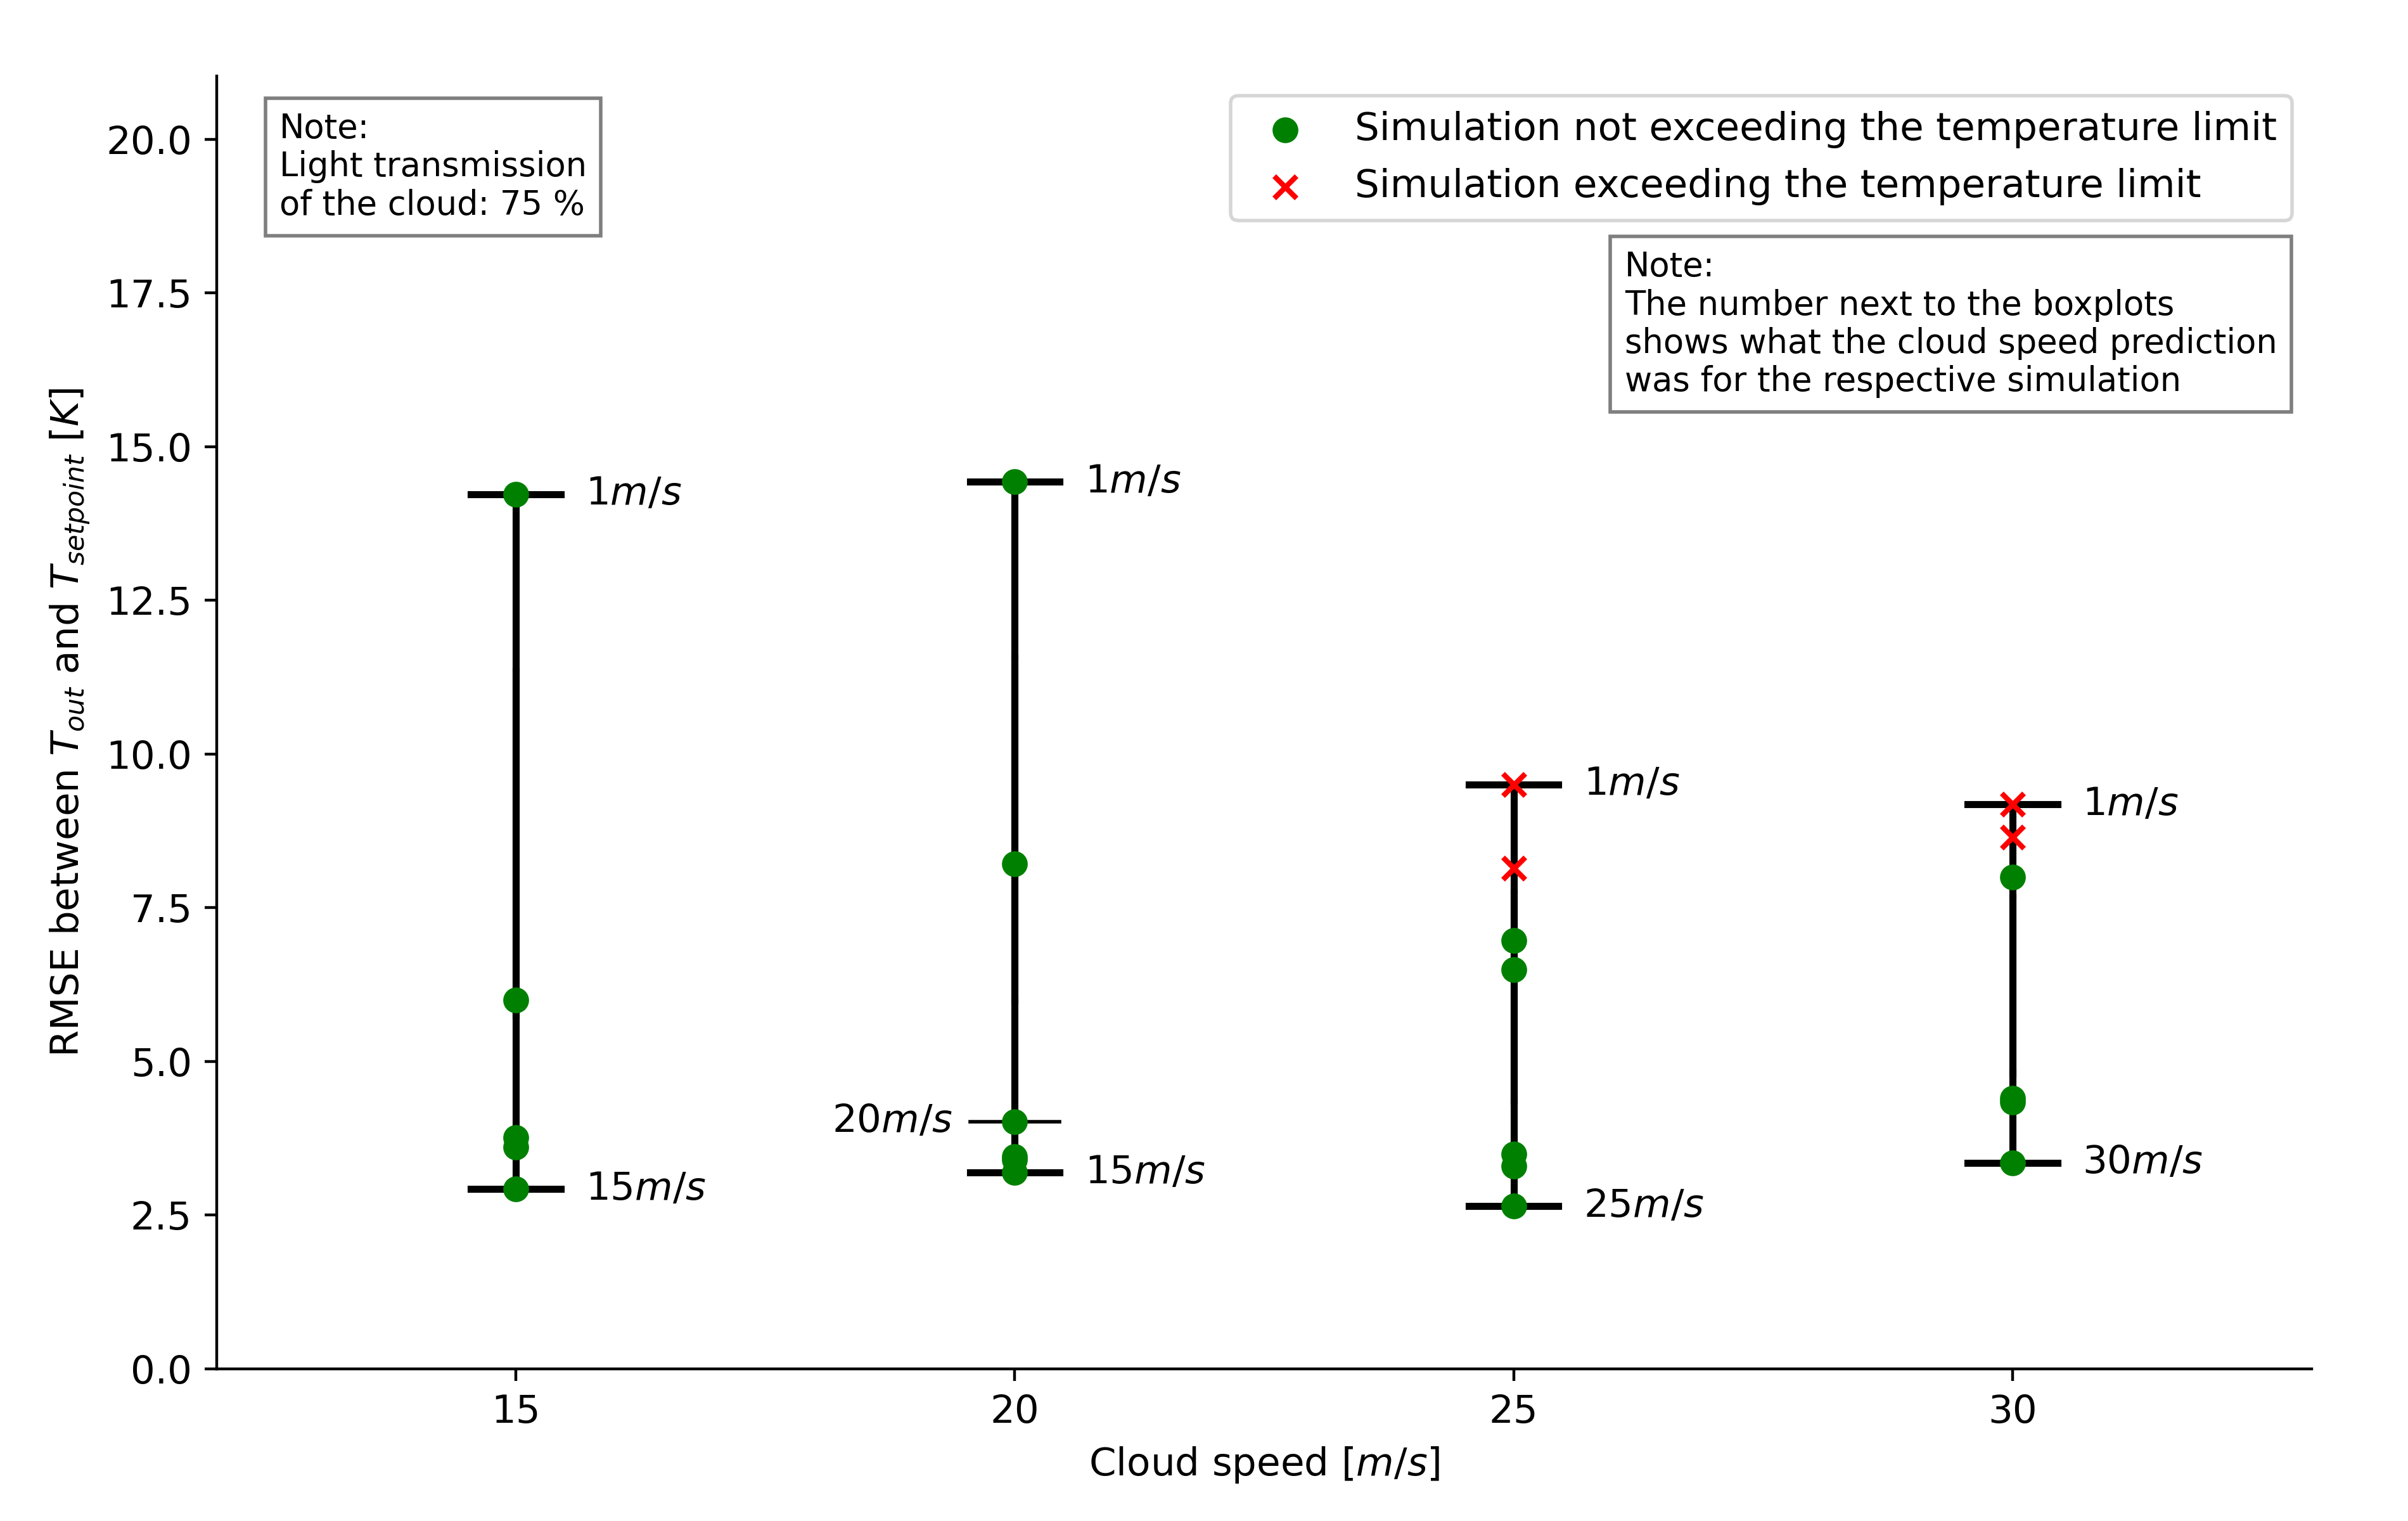
\includegraphics[width=0.89\textwidth]{C:/Users/gesc_ma/VSCode MPC Projekt/dynaovrcontroller/dynaovrcontroller/aimpoint_control_scenarios/plots/21_analyze_speed_uncertainty/rmse_per_speed_shading_75.png}}
    \caption[Analyse des RMSE für unterschiedliche Prädiktionen der Wolkengeschwindigkeiten für eine Lichtdurchlässigkeit der Wolke von $\SI{75}{\percent}$]{Analyse des RMSE für unterschiedliche Prädiktionen der Wolkengeschwindigkeiten für eine Lichtdurchlässigkeit der Wolke von $\SI{75}{\percent}$}
    \label{fig_speed75RMSE}
\end{figure}

\begin{figure}[t]
    \centering
    \setlength{\fboxsep}{1pt}
    \setlength{\fboxrule}{1pt}
    \fbox{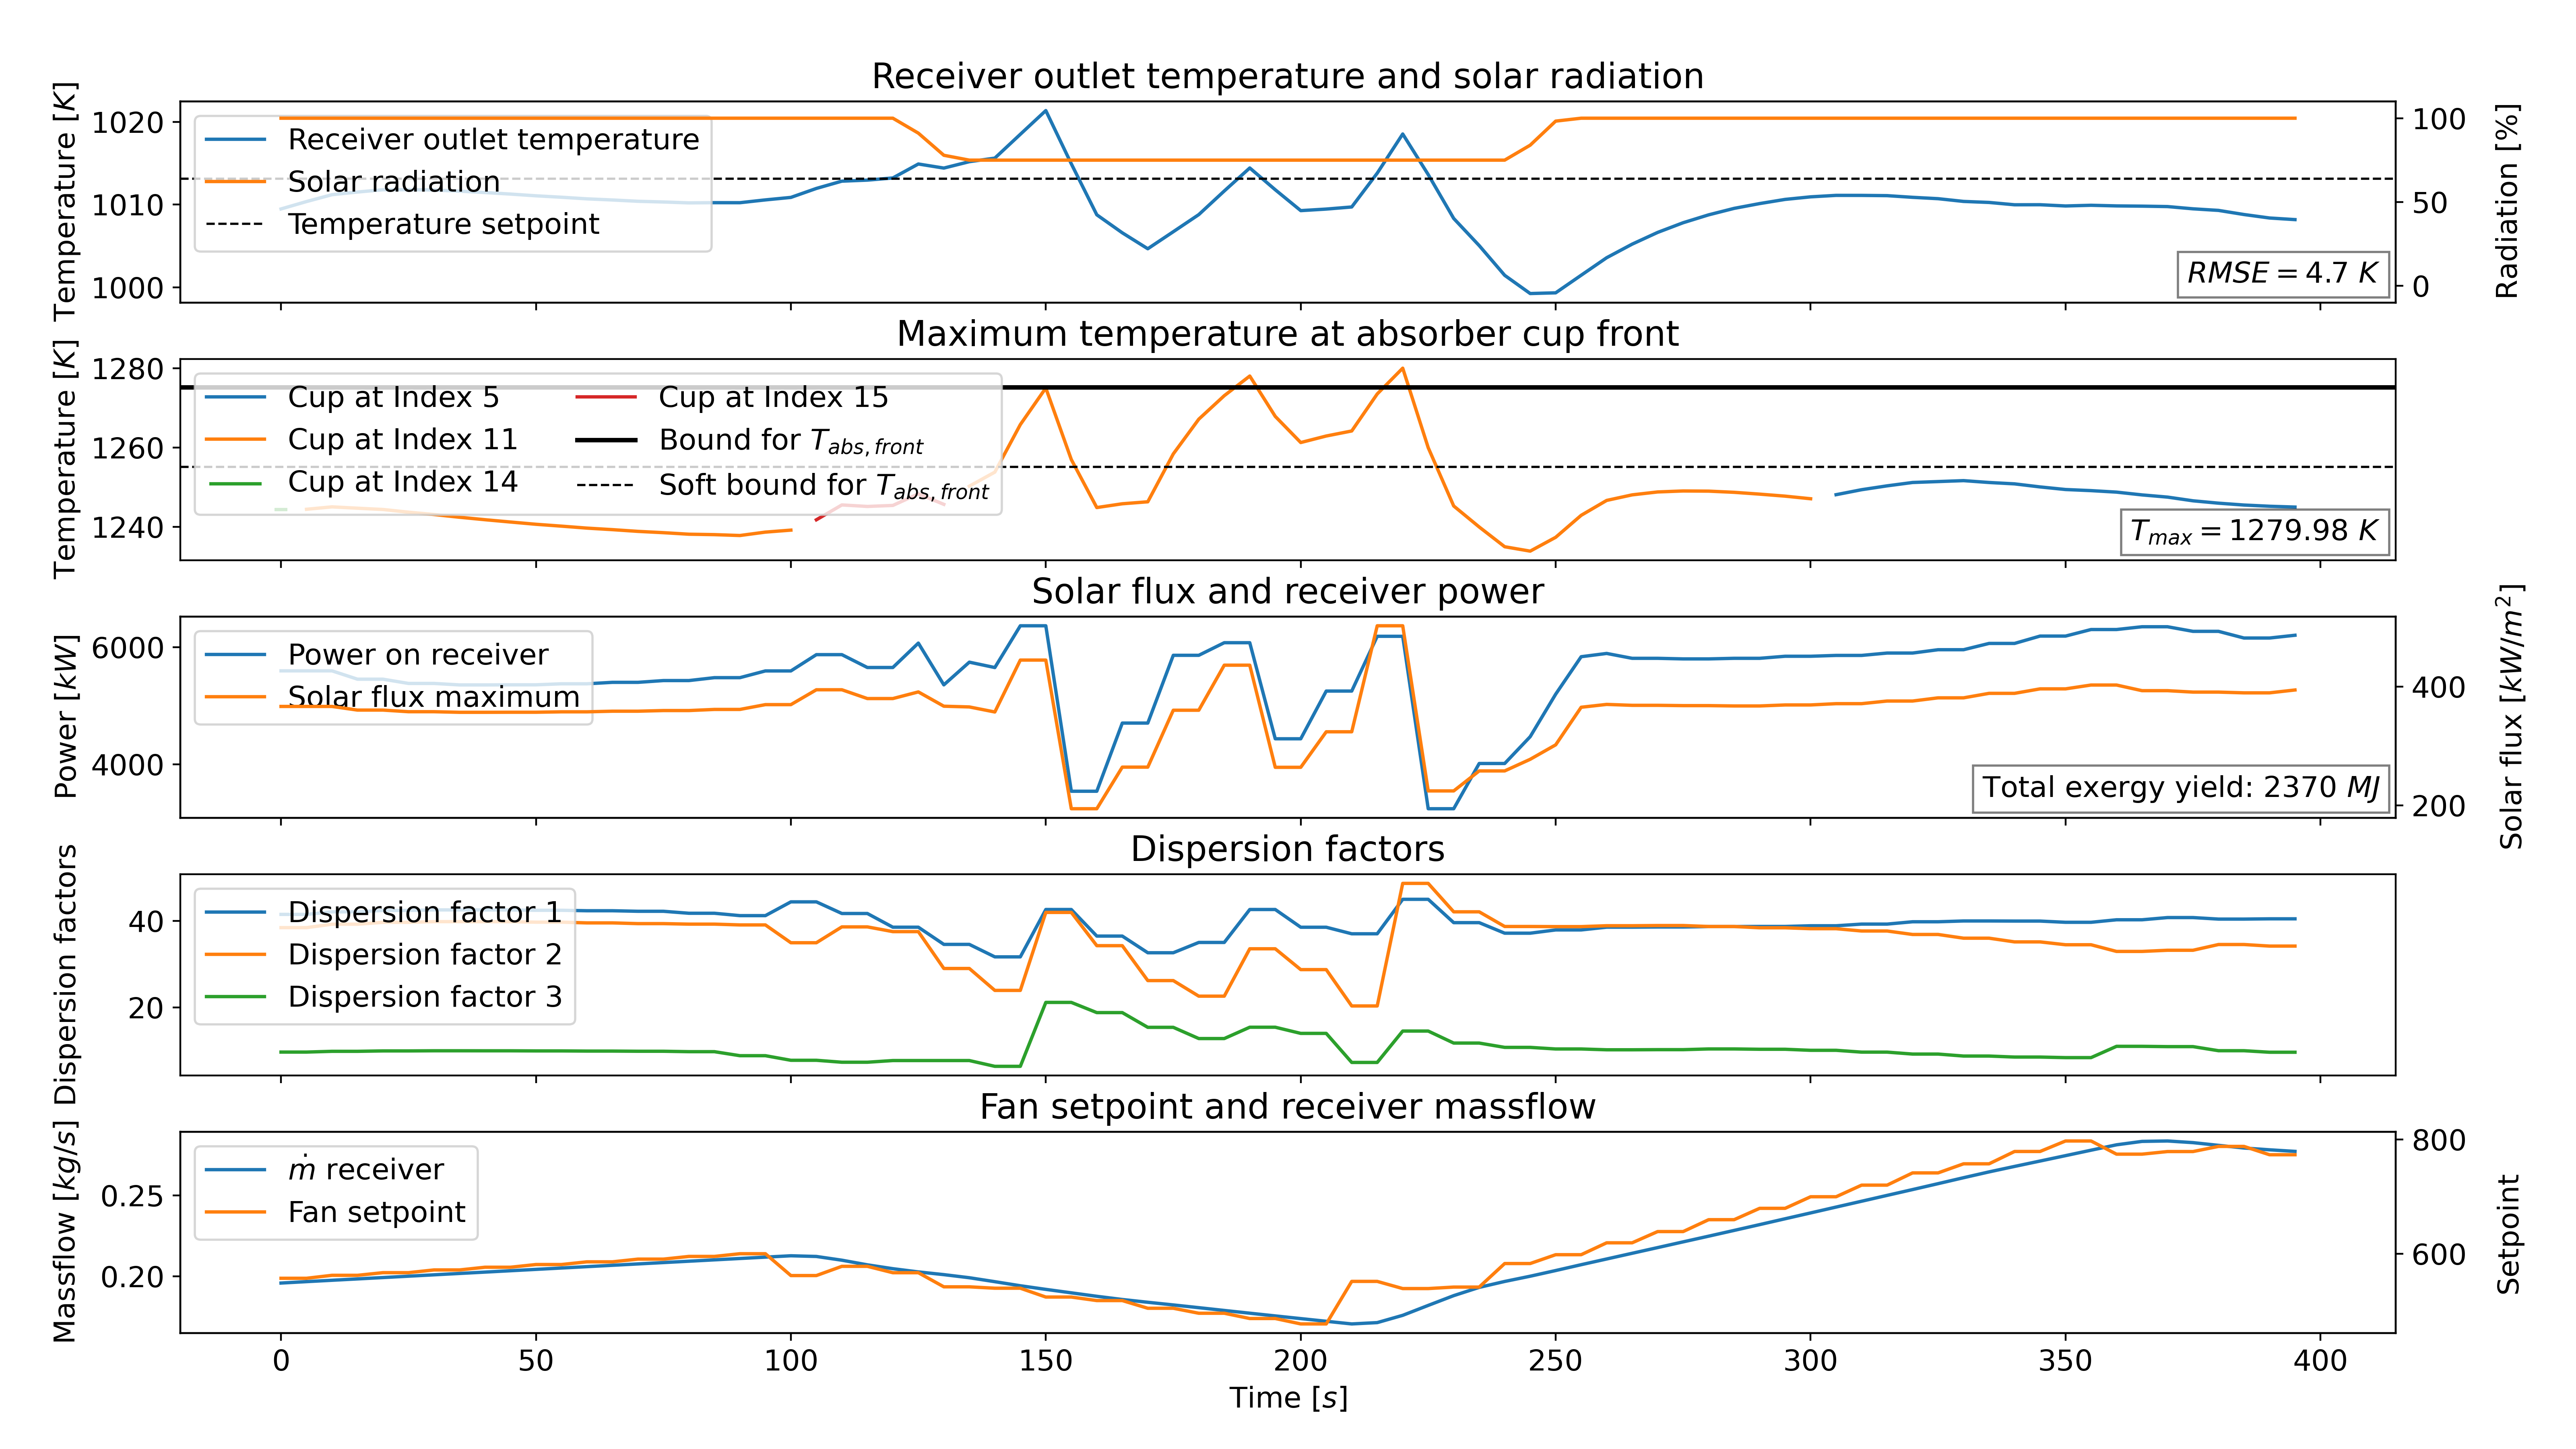
\includegraphics[width=0.99\textwidth]{C:/Users/gesc_ma/VSCode MPC Projekt/dynaovrcontroller/dynaovrcontroller/aimpoint_control_scenarios/plots/04_mpc_uncertain_information_shading/75/shading_120sec_75_30mps_thinking_50.png}}
    \caption[Simulationsverlauf mit Wolkengeschwindigkeit $\SI{30}{\metre\per\second}$ von Lichtdurchlässigkeit von $\SI{75}{\percent}$ bei Vorhersage von $\SI{0}{\percent}$]{Simulationsverlauf mit Wolkengeschwindigkeit $\SI{30}{\metre\per\second}$ von Lichtdurchlässigkeit von $\SI{75}{\percent}$ bei Vorhersage von $\SI{0}{\percent}$}
    \label{fig_uncertain753000}
 \end{figure}
							% Anhang


\end{document}